\documentclass[reqno]{amsart}
\usepackage[utf8]{inputenc}
\usepackage[margin=1in]{geometry}
\usepackage[usenames, dvipsnames]{xcolor}
\usepackage{graphicx}
\usepackage{mathtools}
\usepackage{amssymb}
\usepackage{amsthm}
\usepackage{fancyhdr}
\usepackage{adforn}
\usepackage{xparse}
\usepackage{tikz}
\usetikzlibrary{fadings}
%\usetikzlibrary{matrix, positioning, calc}
% Additional math macros that I want in both my notes and my psets
\usepackage[sc, noBBpl]{mathpazo}
\usepackage{mathrsfs}
\usepackage[T1]{fontenc}
\usepackage{calligra}
\usepackage{microtype}
\usepackage[all]{xy}
\usepackage{slashed}
\newcommand{\A}{\mathbb A}
\newcommand{\cat}{\mathsf}
\newcommand{\sC}{\cat C}
\newcommand{\sD}{\cat D}
\newcommand{\sS}{\cat S}
\newcommand{\sA}{\mathscr A}
\newcommand{\sF}{\mathscr F}
\newcommand{\sG}{\mathscr G}
\renewcommand{\P}{\mathbb P}
\newcommand{\cO}{\mathscr O}
\newcommand{\sI}{\mathscr I}
\DeclareMathOperator{\coker}{coker}
\renewcommand{\Im}{\operatorname{Im}}
\newcommand{\pt}{\mathrm{pt}}
\DeclareMathOperator{\Hom}{Hom}
\newcommand{\op}{^{\mathsf{op}}}
\newcommand{\Id}{\mathrm{Id}}
\DeclareMathOperator{\Mat}{Mat}
\newcommand{\m}{\mathfrak m}
%\newcommand{\p}{\mathfrak p}
\newcommand{\q}{\mathfrak q}
\DeclareMathOperator{\MSpec}{MSpec}
\DeclareMathOperator{\Spec}{Spec}
\newcommand{\Top}{\cat{Top}}
\newcommand{\Ring}{\cat{Ring}}
\newcommand{\Mod}{\cat{Mod}}
\DeclareMathOperator{\res}{res}
\newcommand{\Alg}{\cat{Alg}}
\newcommand{\Fun}{\cat{Fun}}
\newcommand{\AffSch}{\cat{AffSch}}
\newcommand{\Ab}{\cat{Ab}}
\DeclareMathOperator{\bl}{--}
\DeclareMathOperator{\Free}{Free}
\DeclareMathOperator{\For}{For}
\newcommand{\Set}{\cat{Set}}
\newcommand{\LocRing}{\cat{LocRing}}
\newcommand{\Grp}{\cat{Grp}}
\newcommand{\Sch}{\cat{Sch}}
\newcommand{\inHom}{\operatorname{\underline{\Hom}}}
\DeclareMathOperator{\Frac}{Frac}
\DeclareMathOperator{\Gal}{Gal}
\DeclareMathOperator{\Nil}{Nil}
\newcommand{\pre}{\sC^{\text{pre}}}
\newcommand{\sh}{_{\text{sh}}}
\newcommand{\G}{\mathbb G}
\DeclareMathOperator{\Proj}{Proj}
\newcommand{\sM}{\mathscr M}
\newcommand{\sV}{\mathscr V}
\newcommand{\fU}{\mathfrak U}
\newcommand{\GL}{\mathrm{GL}}
\DeclareMathOperator{\Sym}{Sym}
% http://tex.stackexchange.com/questions/141434/how-to-type-sheaf-hom
\DeclareMathOperator{\shom}{\mathscr{H}\text{\kern -4pt {\calligra\large om}}\,}
\newcommand{\sL}{\mathscr L}
\DeclareMathOperator{\QC}{QC}
\DeclareMathOperator{\Supp}{Supp}
\newcommand{\sN}{\mathscr N}
\DeclareMathOperator{\Ann}{Ann}
\DeclareMathOperator{\Der}{Der}
\newcommand{\ctcpx}[1]{(#1)^{\text{der}}}
\newcommand{\Dist}{\mathsf{Dist}}
\newcommand{\shdi}{\operatorname{Sh}_{\Dist}}
\DeclareMathOperator{\Sh}{Sh}
\newcommand{\shz}{\mathsf{Sh}_{\text{\rm Zar}}}
\DeclareMathOperator{\Gr}{Gr}
% Source: http://tug.org/pipermail/xy-pic/2001-July/000015.html
\newcommand{\pullbackcorner}[1][dr]{\save*!/#1+1.2pc/#1:(1,-1)@^{|-}\restore}
\newcommand{\pushoutcorner}[1][dr]{\save*!/#1-1.2pc/#1:(-1,1)@^{|-}\restore}
\newcommand{\TDel}{\mathrm{2\Delta}}
\DeclareMathOperator{\Bl}{B\ell}
\newcommand{\cR}{\mathcal R}
\newcommand{\cL}{\mathcal L}
\newcommand{\cH}{\mathcal H}
\newcommand{\refR}{\reflectbox{\(\cR\)}}

\renewcommand{\a}{\alpha}
\renewcommand{\b}{\beta}
%\newcommand{\e}{\epsilon}
\renewcommand{\l}{\lambda}
\renewcommand{\L}{\Lambda}
\newcommand{\g}{\gamma}
\newcommand{\s}{\sigma}
\newcommand{\z}{\zeta}
\newcommand{\RR}{\mathbb{R}}
\newcommand{\NN}{\mathbb{N}}
\newcommand{\QQ}{\mathbb{Q}}
\newcommand{\ZZ}{\mathbb{Z}}
\newcommand{\CC}{\mathbb{C}}
\newcommand{\cC}{\mathcal{C}}
\newcommand{\f}{\frac}
\newcommand{\p}{\partial}
\renewcommand{\P}[3][]{\f{\partial^{#1} #2}{\partial #3 ^{#1}}}
%\newcommand{\avg}[1]{\langle #1 \rangle}
\newcommand{\avg}[1]{\left< #1 \right>}
\newcommand{\?}{\overset{?}{=}}
\newcommand{\Int}{\int_{-\infty}^\infty}
\newcommand{\ket}[1]{\left| #1 \right>} % for Dirac bras
\newcommand{\bra}[1]{\left< #1 \right|} % for Dirac kets
\newcommand{\braket}[2]{\left< #1 \vphantom{#2} \right|
 \left. #2 \vphantom{#1} \right>} % for Dirac brackets
\newcommand{\pv}{\vec{p}}

\newcommand{\grad}[1]{\gv{\nabla} #1} % for gradient
\let\divsymb=\div % rename builtin command \div to \divsymb
\renewcommand{\div}[1]{\gv{\nabla} \cdot #1} % for divergence
\newcommand{\curl}[1]{\gv{\nabla} \times #1} % for curl
\renewcommand{\labelenumi}{(\alph{enumi})}
\let\vaccent=\v % rename builtin command \v{} to \vaccent{}
\renewcommand{\v}[1]{\ensuremath{\mathbf{#1}}}
\newcommand{\uv}[1]{\ensuremath{\mathbf{\hat{#1}}}} % for unit vector
\newcommand{\gv}[1]{\ensuremath{\mbox{\boldmath$ #1 $}}} 
% for vectors of Greek letters
\usepackage{hyperref}
\usepackage{siunitx}

%\usepackage[compat=1.1.0]{tikz-feynman}

% TODO fiddle with colors
\definecolor{newblue}{HTML}{1F98A6}
\definecolor{newred}{HTML}{D95448}
\definecolor{neworange}{HTML}{F29441}
\hypersetup{
	colorlinks,
	linkcolor=newred,
	citecolor=neworange,
	urlcolor=newblue!80!black,
}
\usepackage[all]{hypcap}
\pagestyle{plain}
\setcounter{tocdepth}{1}


\usepackage{titlesec}
\titleformat{\section}[frame]
  {\normalfont}
  {\filright
   \footnotesize
   \enspace Lecture \arabic{section}.\enspace}
  {8pt}
  {\Large\bfseries\filcenter}
\usepackage[dotinlabels]{titletoc}
\titlecontents{section}[1.5em]{}{\contentslabel{2.3em}}{\hspace*{-2.3em}}{\hfill\contentspage}

\renewcommand{\sectionmark}[1]{\markleft\thesection. #1}

\fancyhf{}
\fancyhead[RO,LE]{\small\thepage}
\fancyhead[LO]{\small\slshape\nouppercase{\rightmark}}
\fancyhead[RE]{\small\slshape Advanced Quantum Field Theory Lecture Notes}
\setlength{\headheight}{11.0pt}
\pagestyle{fancy}

\numberwithin{equation}{section}
\newcommand{\orbreak}{
\begin{center}
	\adforn{17}\;\(\cdot\)\;\adforn{18}
	\vspace{0.2cm}
\end{center}
}

\renewcommand{\labelitemi}{\(\circ\)}

% I wanted to allow one to reference parts of a thm/cor/etc. and have it print the thm number too, e.g. 29.2(1),
% but this isn't working right now. Probably the best way to do this would be to play around with enumitem to
% define a new enumerate-like counter and then just use that directly instead of enumerate in comp.

% This feels really wobbly, but so far it's working
\NewDocumentEnvironment{comp}{mm}{%
	\csname #1\endcsname\hfill
	\csname #2\endcsname
}{
	\csname end#2\endcsname
	\csname end#1\endcsname
}

% usage:
% \shortexact[f][g]{A}{B}{C},
%
%			 f    g
% for 0 -> A -> B -> C -> 0,
\DeclareDocumentCommand{\shortexact}{O{} O{} mmmm}{
\xymatrix{
	0\ar[r] & #3\ar[r]^-{#1} & #4\ar[r]^-{#2} & #5\ar[r] & 0#6
}}
% exactly the same, but for 0 -> A -> B -> C
\DeclareDocumentCommand{\leftexact}{O{} O{} mmmm}{
\xymatrix{
	0\ar[r] & #3\ar[r]^-{#1} & #4\ar[r]^-{#2} & #5 #6
}}
% ... and the same, for A -> B -> C -> 0
\DeclareDocumentCommand{\rightexact}{O{} O{} mmmm}{
\xymatrix{
	#3\ar[r]^-{#1} & #4\ar[r]^-{#2} & #5\ar[r] & 0#6
}}



% usage:
% X\dblarrow[r] & Y
%   f
% X => Y
%   g
\DeclareDocumentCommand{\dblarrow}{O{} O{} O{}}{
	\ar@<0.4ex>[#1]^-{#2}\ar@<-0.4ex>[#1]_-{#3}
}
% Note: it would be a useful exercise to figure out how to define this so it can be used as
% \dblarrow[r]^f_g

\everyentry={\displaystyle}

\newcommand{\N}{\mathbb N}
\newcommand{\Z}{\mathbb Z}
\newcommand{\Q}{\mathbb Q}
\newcommand{\R}{\mathbb R}
\newcommand{\C}{\mathbb C}
\newcommand{\F}{\mathbb F}
\newcommand{\vp}{\varphi}
\newcommand{\term}{\emph}
\renewcommand{\vec}[1]{\boldsymbol{\mathbf{#1}}}
\DeclarePairedDelimiter\paren{(}{)}
%\DeclarePairedDelimiter\ang{\langle}{\rangle}
\DeclarePairedDelimiter\abs{\lvert}{\rvert}
\DeclarePairedDelimiter\norm{\lVert}{\rVert}
\DeclarePairedDelimiter\bkt{[}{]}
\DeclarePairedDelimiter\set{\{}{\}}
% Swap paren* and paren, etc., so that the normal version resizes by default.
% Meanwhile, one can use \paren*[\Big]{...} to customize the size easily.
% It would be interesting to wrap this up into a custom \definedelimiter command...
\makeatletter
	\let\oldparen\paren
	\def\paren{\@ifstar{\oldparen}{\oldparen*}}
	\let\oldbkt\bkt
	\def\bkt{\@ifstar{\oldbkt}{\oldbkt*}}
\makeatother
\newcommand{\e}{\varepsilon}
\def\qedsymbol{{\small{\ensuremath{\boxtimes}}}}
\newcommand{\inj}{\hookrightarrow}
\newcommand{\surj}{\twoheadrightarrow}
\DeclareMathOperator{\id}{id}
\newcommand{\ud}{\,\mathrm{d}}
\renewcommand{\d}{\mathrm d}
\newcommand{\dfr}[2]{\frac{\mathrm d #1}{\mathrm d #2}}
\newcommand{\pfr}[2]{\frac{\partial #1}{\partial #2}}

%\catcode`\"=13
%\newcommand{"}[1]{^{(#1)}}
\newtheorem{thm}[equation]{Theorem}
\newtheorem*{thm*}{Theorem}
\newtheorem{lem}[equation]{Lemma}
\newtheorem*{lem*}{Lemma}
\newtheorem{cor}[equation]{Corollary}
\newtheorem{prop}[equation]{Proposition}
\newtheorem{obs}[equation]{Observation}
\theoremstyle{definition}
\newtheorem{ex}[equation]{Exercise}
\newtheorem{exm}[equation]{Example}
\newtheorem{defn}[equation]{Definition}
\newtheorem*{claim}{Claim}
\theoremstyle{remark}
\newtheorem*{rem}{Remark}
\newtheorem*{fct}{Fact}
\newtheorem*{note}{Note}

\begin{document}
\title{Supersymmetry}
\author{Ian Lim\\ Last updated \today}
\maketitle
{\small\noindent These notes were taken for the \textit{Supersymmetry} course taught by D. Skinner at the University of Cambridge as part of the Mathematical Tripos Part III in Lent Term 2019. I live-\TeX ed them using Overleaf, and as such there may be typos; please send questions, comments, complaints, and corrections to 
\href{mailto:itel2@cam.ac.uk?subject=SUSY\%20Lecture\%20Notes}{\texttt{itel2@cam.ac.uk}}.\\
Many thanks to Arun Debray for the {\LaTeX} template for these lecture notes: as of the time of writing, you can find him at \url{https://web.ma.utexas.edu/users/a.debray/}.}

\tableofcontents

\section{Tuesday, January 22, 2019}
    Last time, we introduced the path integral in quantum mechanics, and we said it took the form
\begin{equation}
    \bra{x}e^{-iHt/\hbar}\ket{x_0}=\int \cD x e^{iS[x]/\hbar}.
\end{equation}
Let us consider now a ``rotation'' to imaginary time, $t\to - i\tau$ (Wick rotation). Then our path integral becomes
\begin{equation}
    \bra{x}e^{-H\tau/\hbar}\ket{x_0}=\int \cD x e^{-S[x]/\hbar}.
\end{equation}
Working with a real exponent has some benefits-- the convergence of the integral is more obvious, and in the $\hbar \to 0$ limit we expect the integral to be dominated by the classical path $x$ which minimizes the action $S[x].$

We can now observe that 1D quantum mechanics is like a $0+1$D quantum field theory-- the field is simply
\begin{equation*}
    x(t): \RR \to \RR.
\end{equation*}
In fact, 3D quantum mechanics is also like a $0+1$D QFT, where the field is now
\begin{equation*}
    \vec x(t): \RR \to \RR^3.
\end{equation*}
Given a single spacetime label $t$, a QM theory gives us a real scalar in $\RR$ or a vector in $\RR^3$-- cf. Srednicki Ch. 1. There are different approaches to quantization, but in the \term{second quantization} formalism we demote position $\vec x$ from an operator $\hat x$ to a label on a spacetime point $(\vec x,t)$. Therefore QFT in $3+1$ dimensions has e.g. a scalar field $\phi$ which is a map
\begin{equation*}
    \phi: \RR^{1,3}\to \RR.
\end{equation*}

\subsection*{Path integral methods}
Let's begin with the simplest possible case, QFT in zero dimensions.%
    \footnote{Cf. Skinner Ch. 2, Srednicki \textsection 8,9.}
All of spacetime is a single point $p$,%
    \footnote{If you're reading my SUSY notes, you should be getting d\'ej\`a vu right about now.}
and our (real scalar) field $\phi$ is a map $\phi:\set{p}\to\RR$.

Using our imaginary time (Euclidean signature) convention for the path integral, we write
\begin{equation}
    Z = \int_\RR d\phi\, e^{-S[\phi]/\hbar}.
\end{equation}
We'll take our action $S[\phi]$ to be polynomial in $\phi$, with highest power even.

As in statistical field theory, we are interested in correlation functions and expectation values. Given a function $f(\phi)$, we might like to compute the expectation value
\begin{equation}
    \avg{f}=\frac{1}{Z} \int d\phi \, f(\phi)e^{-S[\phi]/\hbar}.
\end{equation}
For this to have a chance of convergence, $f$ should not grow too rapidly as $|\phi| \to \infty$. Usually the functions we are interested in are polynomial in $\phi$.

\subsection*{Free field theory}
Suppose we have $N$ real scalar fields $\phi_a, a=1,\ldots, N$. We can compactly write this as a single field
\begin{equation}
    \phi: \set{p}\to \RR^N,
\end{equation}
and we'd like to compute the integral
\begin{equation}
    Z_0 = \int d^N\, \phi e^{-S[\phi]/\hbar}.
\end{equation}
Now, a free theory simply means that the action is quadratic in our fields. A priori it could have included kinetic terms, but since we are in zero dimensions, there are no derivatives to take and therefore no kinetic terms in this model. Then we can write our action as
\begin{equation}
    S(\phi)=\frac{1}{2} \cM_{ab} \phi_a \phi_b =\frac{1}{2} \phi^T \cM \phi,
\end{equation}
where $\cM$ is an $N\times N$ symmetric matrix with $\det M > 0$. So our action could include terms like $\frac{1}{2}\phi_1^2$ and $\frac{5}{2} \phi_1 \phi_4$. Since $\cM$ is symmetric, we can diagonalize it as
\begin{equation*}
    \cM=P\Lambda P^T
\end{equation*}
for some orthogonal matrix $P$. But equivalently we could just redefine our fields to some new fields $\phi'= P^T  \phi$ so that 
\begin{equation*}
    S(\phi)= \frac{1}{2} \phi'{}^T \Lambda \phi'= \frac{1}{2} \sum_{i=1}^N \lambda_i (\phi'_i)^2,
\end{equation*}
where $\lambda_i$ are the eigenvalues of $\cM$. Since $P$ is orthogonal, $\det P = 1 \implies d^N \phi=(\det P)d^N \phi' = d^N \phi'$, so our path integral separates into $N$ Gaussian integrals of the form
\begin{equation}
    \int_{-\infty}^\infty dx\, e^{-\frac{\lambda}{2\hbar}x^2}=\sqrt{\frac{2\pi \hbar}{\lambda}}.
\end{equation}
Thus
\begin{equation}
    Z_0 = \int d^N \phi \, e^{-\frac{1}{2\hbar}\phi^T \cM \phi}= \prod_{i=1}^N d \phi_i \, e^{-\frac{1}{2\hbar} \lambda_i (\phi_i)^2} = \frac{(2\pi \hbar)^{N/2}}{\sqrt{\det \cM}}.
\end{equation}

We can now  introduce a source term $J$, modifying our action to
\begin{equation}
    S(\phi)=\frac{1}{2} \phi^T \cM \phi + J\cdot \phi.
\end{equation}
If we complete the square and make a change of variables $\tilde \phi= \phi+ \cM^{-1} J,$
we find that the new path integral with a source is
\begin{align*}
    Z_0[J] &= \int d^N \phi \, \exp \bkt{-\frac{1}{2\hbar} \phi^T \cM \phi -\frac{1}{\hbar} J \cdot \phi}\\
        &= \exp\paren{\frac{1}{2\hbar}J^T \cM^{-1} J} \int d^N \tilde \phi\, e^{-\frac{1}{2\hbar} \tilde \phi^T \cM \tilde \phi}\\
        &= Z_0 \exp\paren{\frac{1}{2\hbar} J^T \cM^{-1} J}.
\end{align*}
We see that $\P{}{J}$ derivatives will bring down $\phi$s, which will allow us to compute correlation functions just like we did in statistical physics with the partition function.

\begin{exm}
    What is the value of the correlation function $\avg{\phi_a \phi_b}$ in this theory? We can compute it directly:
    \begin{align*}
        \avg{\phi_a \phi_b} &= \frac{1}{Z_0}\left.\int d^N \phi \, \phi_a \phi_b \exp\bkt{-\frac{1}{2\hbar} \phi^T \cM \phi -\frac{1}{\hbar} J \cdot \phi}\right|_{J=0}\\
            &= \frac{1}{Z_0} \int d^N \phi \paren{-\hbar \P{}{J_a}} \paren{-\hbar \P{}{J_b}} \left.\exp \bkt{-\frac{1}{2\hbar} \phi^T \cM \phi -\frac{1}{\hbar} J \cdot \phi}\right|_{J=0}\\
            &= (-\hbar)^2 \P{}{J_a}\P{}{J_b} \left.\exp\bkt{\frac{1}{2\hbar} J^T \cM^{-1} J}\right|_{J=0}\\
            &= \hbar (\cM^{-1})_{ab}.
    \end{align*}
    Note that the first $J$ derivative brings down an $\cM^{-1}J$ (so our expression is of the form $\cM^{-1} J \exp (J^T \cM^{-1} J)$), and when we take the second $J$ derivative, we will get two terms, one of the form $\cM^{-1}\exp(\ldots)$ and another of the form $(\cM^{-1}J)^2 \exp(\ldots)$. The second term is zero when we set $J=0$, and the exponential becomes $1$ in both cases, so we are just left with $\cM^{-1}$. 
\end{exm}
What we have calculated is a two-point function, otherwise known as a propagator (though it's a bit silly to call this a propagator when the spacetime is just a single point). We can associate a Feynman diagram to this process:
%
\begin{center}
    \begin{tikzpicture}[x=0.75pt,y=0.75pt,yscale=-1,xscale=1]
        
        %Straight Lines [id:da8887105125657073] 
        \draw    (200,123) -- (260,123) ;
        \draw  [color={black}  ][fill={black}  ][line width=0.75]      (200, 123) circle [x radius= 3.35, y radius= 3.35]   ;
        \draw  [color={black}  ][fill={black}  ][line width=0.75]      (260, 123) circle [x radius= 3.35, y radius= 3.35]   ;
        
        % Text Node
        \draw (200,106) node  [align=left] {a};
        % Text Node
        \draw (260,106) node  [align=left] {b};
    
    \end{tikzpicture}
\end{center}

There is another method we can use to compute propagators (cf. Osborn \textsection 1.3):
\begin{align*}
    \cM_{ca} \avg{\phi_a \phi_b} &= \frac{1}{Z_0} 
        \int d^N \phi \,\cM_{ca} \phi_a \phi_b \exp\bkt{-\frac{1}{2\hbar} \phi^T \cM \phi}\\
        &= -\frac{\hbar}{Z_0} \int d^N \phi \, \phi_b \P{}{\phi_c} \exp\bkt{-\frac{1}{2\hbar} \phi^T \cM \phi}\\
        &= \frac{\hbar}{Z_0}\int d^N \phi\, \P{\phi_b}{\phi_c} \exp\bkt{-\frac{1}{2\hbar} \phi^T \cM \phi}\\
        &= \hbar \delta_{bc} \implies \avg{\phi_a \phi_b}=\hbar (\cM^{-1})_{ab}.
\end{align*}
In going from the second to the third line, we have integrated by parts to move the $\P{}{\phi_c}$ to $\phi_b,$ and then recognized the remaining integral as $Z_0$.

More generally, let $l(\phi)= l \cdot \phi = \sum_{a=1}^N l_a \phi_a (\neq 0)$ be a linear function of $\phi$, with $l_a \in \RR.$ Then the expected value $\avg{l_a(\phi) \ldots l_p(\phi)}$ is given by
\begin{equation*}
    \avg{l_a(\phi) \ldots l_p(\phi)} = 
        (-\hbar)^p \prod_{i=1}^p \paren{l_i \P{}{J_i}} \left.\frac{Z_0[J]}{Z_0}\right|_{J=0}.
\end{equation*}

Notice that if we play this game for an odd number of $J_i$ derivatives, all our terms will be of the form $J^p \exp(\ldots)$ where $p$ is odd. When we set $J=0$, all these terms therefore vanish, which tells us that $\avg{\phi_{a_1}\ldots \phi_{a_p}}=0$ for $n$ odd. If we compute it for $p=2k, k\in \NN$, the terms that survive setting $J=0$ will have $k$ factors of $\cM^{-1}$.

\begin{exm}
    What is the value of the four-point function $\avg{\phi_a \phi_b \phi_c \phi_d}$ in free field theory? It is simply
    \begin{equation*}
        \avg{\phi_a \phi_b \phi_c \phi_d} =\hbar^2 \bkt{(\cM^{-1})_{ab} (\cM^{-1})_{cd} + (\cM^{-1})_{ac} (\cM^{-1})_{bd} + (\cM^{-1})_{ad} (\cM^{-1})_{bc}}.
    \end{equation*}
    Though we haven't said it, this is effectively a toy version of Wick's theorem-- we are taking contractions of the fields using $(\cM^{-1})$s as propagators.
    
    We can depict these contractions as connecting some $2k$ dots pairwise with lines using a simplified Feynman diagram notation:
    
    \begin{center}
    \begin{tikzpicture}[x=0.75pt,y=0.75pt,yscale=-1,xscale=1]
    %uncomment if require: \path (0,300); %set diagram left start at 0, and has height of 300
        
        %Straight Lines [id:da8887105125657073] 
        \draw    (100,123) -- (160,123) ;
        \draw [shift={(100,123)}, rotate = 0] [color={black}  ][fill={black}  ][line width=0.75]      (0, 0) circle [x radius= 3.35, y radius= 3.35]   ;
        \draw [shift={(160,123)}, rotate = 0] [color={black}  ][fill={black}  ][line width=0.75]      (0, 0) circle [x radius= 3.35, y radius= 3.35]   ;
        
        % Text Node
        \draw (100,106) node  [align=left] {a};
        % Text Node
        \draw (160,106) node  [align=left] {b};
        
        %Straight Lines [id:da8887105125657073] 
        \draw    (100,173) -- (160,173) ;
        \draw [shift={(100,173)}, rotate = 0] [color={black}  ][fill={black}  ][line width=0.75]      (0, 0) circle [x radius= 3.35, y radius= 3.35]   ;
        \draw [shift={(160,173)}, rotate = 0] [color={black}  ][fill={black}  ][line width=0.75]      (0, 0) circle [x radius= 3.35, y radius= 3.35]   ;
        
        % Text Node
        \draw (100,186) node  [align=left] {c};
        % Text Node
        \draw (160,186) node  [align=left] {d};
        %%end first diagram
        \draw (190,148) node  [align=center] {\huge$+$};
        
        %Straight Lines [id:da8887105125657073] 
        \draw    (220,123) -- (220,173) ;
        \draw [shift={(220,123)}, rotate = 0] [color={black}  ][fill={black}  ][line width=0.75]      (0, 0) circle [x radius= 3.35, y radius= 3.35]   ;
        \draw [shift={(280,123)}, rotate = 0] [color={black}  ][fill={black}  ][line width=0.75]      (0, 0) circle [x radius= 3.35, y radius= 3.35]   ;
        
        % Text Node
        \draw (220,106) node  [align=left] {a};
        % Text Node
        \draw (280,106) node  [align=left] {b};
        
        %Straight Lines [id:da8887105125657073] 
        \draw    (280,123) -- (280,173) ;
        \draw [shift={(220,173)}, rotate = 0] [color={black}  ][fill={black}  ][line width=0.75]      (0, 0) circle [x radius= 3.35, y radius= 3.35]   ;
        \draw [shift={(280,173)}, rotate = 0] [color={black}  ][fill={black}  ][line width=0.75]      (0, 0) circle [x radius= 3.35, y radius= 3.35]   ;
        
        % Text Node
        \draw (220,186) node  [align=left] {c};
        % Text Node
        \draw (280,186) node  [align=left] {d};
        %%end second diagram
        \draw (310,148) node  [align=center] {\huge$+$};
        
        %Straight Lines [id:da8887105125657073] 
        \draw    (340,123) -- (400,173) ;
        \draw [shift={(340,123)}, rotate = 0] [color=black  ][fill={black}  ][line width=0.75]      (0, 0) circle [x radius= 3.35, y radius= 3.35]   ;
        \draw [shift={(400,123)}, rotate = 0] [color={black}  ][fill={black}  ][line width=0.75]      (0, 0) circle [x radius= 3.35, y radius= 3.35]   ;
        
        % Text Node
        \draw (340,106) node  [align=left] {a};
        % Text Node
        \draw (400,106) node  [align=left] {b};
        
        %make the lines look like they cross over
        \draw [shift={(370, 148)}] [color={white}] [fill={white}] (0, 0) circle [x radius= 3.5, y radius= 3.5] ;
        
        %Straight Lines [id:da8887105125657073] 
        \draw    (340,173) -- (400,123) ;
        \draw [shift={(340,173)}, rotate = 0] [color={black}  ][fill={black}  ][line width=0.75]      (0, 0) circle [x radius= 3.35, y radius= 3.35]   ;
        \draw [shift={(400,173)}, rotate = 0] [color={black}  ][fill={black}  ][line width=0.75]      (0, 0) circle [x radius= 3.35, y radius= 3.35]   ;
        
        % Text Node
        \draw (340,186) node  [align=left] {c};
        % Text Node
        \draw (400,186) node  [align=left] {d};
    \end{tikzpicture}
\end{center}
    
    In general, the number of distinct ways we can pair $2k$ elements is
    \begin{equation*}
        \frac{(2k)!}{2^k  k!}.
    \end{equation*}
    The logic here is that we could take all $(2k)!$ permutations of the $2k$ elements, and then take neighboring pairs, e.g. if our elements are $\set{a,b,c,d,e,f}$, one set of pairs is
    \begin{equation*}
        abdcfe\to ab|dc|fe.
    \end{equation*}
    The order of the $2$ elements in each of the $k$ pairs doesn't matter ($ab|dc=ba|dc$), so we've overcounted by a factor of $2^k$, and the order of all the $k$ pairs also doesn't matter ($ab|dc=dc|ab$), so we divide by another factor of $k!$ to get the final result.
\end{exm}

\begin{exm}
    One last example-- if our free fields are instead complex, $\phi:\set{p}\to \CC$, then $\cM$ is hermitian. Therefore $(\cM^{-1})$ will in general not be symmetric, and so the order of the indices matters. That is, $\avg{\phi_a \phi_b^*}=\hbar (\cM^{-1})_{ab}$. Then the associated Feynman diagram has an arrow to indicate direction:
    
    \begin{center}
        \begin{tikzpicture}[x=0.75pt,y=0.75pt,yscale=-1,xscale=1]
            
            %Straight Lines [id:da8887105125657073] 
            \draw    (200,123) -- (260,123) ;
            \draw    (230,118) -- (235,123) -- (230,128);
            \draw  [color={black}  ][fill={black}  ][line width=0.75] (200, 123) circle [x radius= 3.35, y radius= 3.35]   ;
            \draw [color={black}] [fill={black}][line width=0.75]      (260, 123) circle [x radius= 3.35, y radius= 3.35]   ;
            
            % Text Node
            \draw (200,106) node  [align=left] {a};
            % Text Node
            \draw (260,106) node  [align=left] {b};
        
        \end{tikzpicture}
    \end{center}
\end{exm}



\section{Thursday, January 24, 2019}
    Last time, we introduced the Grassman variables. They are a set of elements which anticommute and obey a variation of the Leibniz rule,
\begin{equation*}
    \P{}{\psi^a}(\psi^b \ldots)=\delta^b{}_a (\ldots)-\psi^b \P{}{\psi^a}(\ldots).
\end{equation*}
Of course, now that we've defined differentiation we'd naturally like to define integration as well. Since $(\psi)^2=0$, we only need to define
\begin{equation*}
    \int 1\,d\psi\text{ and } \int \psi d\psi.
\end{equation*}
We want our integral to be ``translation-invariant,'' i.e.
\begin{equation}
    \int (\psi+\eta)d\psi = \int \psi d\eta \implies \int 1 \, d\psi = 0
\end{equation}
for $\eta \in \RR$. We then normalize by choosing
\begin{equation}
    \int \psi d\psi := 1,
\end{equation}
known as \term{Berezin integration}. Suppose we have $n$ fermions $\psi^1, \ldots, \psi^n$, with
\begin{equation}
    \int \psi^1 \psi^2 \ldots \psi^2 \underbrace{d\psi^n d\psi^{n-1}\ldots d \psi^1}_{d^n \psi}=1.
\end{equation}
We must have the $d\psi$s in this order in order to perform each of the integrals, so that
\begin{equation}
    \int \psi^{a_1}\ldots \psi^{a_n}d^n\psi= \epsilon^{a_1a_2\ldots a_n},
\end{equation}
with $\epsilon$ the totally antisymmetric $\epsilon$-symbol.

Now let
\begin{equation}
    \psi'{}^{a}=N^a{}_b \psi^b \text{ for }N\in GL(n).
\end{equation}
We have
\begin{equation}
    \int \psi'{}^a \psi'{}^b \ldots \psi'{}^d d^n \psi = N^a{}_e N^b{}_f \ldots N^d{}_g \int \psi^e \psi^f \ldots \psi^g d^n \psi,
\end{equation}
where we have brought the $N$ ($n\times n$ matrices) by the linearity of the integral-- their entries are just numbers). But indeed we can perform the integral now-- it is
\begin{align*}
    \int \psi'{}^a \psi'{}^b \ldots \psi'{}^d d^n \psi &= N^a{}_e N^b{}_f \ldots N^d{}_g \epsilon^{ef\ldots g}\\
        &= \det(N) \e^{ab\ldots d}\\
        &= \det(N) \int \psi'{}^a \psi'{}^b \ldots \psi'{}^d d^n \psi'.
\end{align*}
Comparing, we see that if $\psi'{}^a=N^a{}_b \psi^b$, then
\begin{equation}
    d^n \psi' = \frac{1}{\det(N)}d^n \psi,
\end{equation}
which is the opposite of the usual convention.

\begin{exm}
    If we have $\chi = a\psi$, then 
    \begin{equation}
        \int \chi d\chi = 1 = a\int \psi d\chi \implies d\chi = \frac{d\psi}{a},
    \end{equation}
    recalling that $\int \psi d\psi =1.$
\end{exm}

For QFT, we often need Gaussian integrals. Suppose $\psi^1,\psi^2$ are fermionic and let
\begin{equation}
    S(\psi)=\frac{1}{2}\psi^1 M \psi^2,
\end{equation}
some sort of action in terms of the fermionic fields $\psi^1,\psi^2$. There are no kinetic terms since we're still working in zero dimensions. Then an integral we might like to calculate is
\begin{equation}
    \int e^{-S(\psi^a)}d \psi^1 d\psi^2.
\end{equation}
But in fact, this integral will be dead simple to calculate. If we Taylor expand the exponential, the expansion actually terminates at the first non-trivial term since the order $(\psi^1 M \psi^2)^2$ term would contain a $(\psi^1)^2$, which vanishes.

Therefore our integral becomes
\begin{equation}
    \int e^{-S(\psi^a)}d \psi^1 d\psi^2 = \int \paren{ (1-\frac{1}{2} \psi^1 M \psi^2
    } d\psi^1 d\psi^2 = \frac{1}{2}M.
\end{equation}
More generally, for $2m$ fermions with ``action'' 
\begin{equation}
    S(\psi^a)=\frac{1}{2} \psi^a M_{ab} \psi^b,
\end{equation}
where we shall take $M_{ab}=-M_{ba}$ to be antisymmetric WLOG, our action integral becomes
\begin{align*}
    \int e^{-S(\psi)}d^{2m}\psi &= \int \sum_{k=0}^\psi \frac{(-1)^k}{k!} \frac{1}{2^k} \paren{\psi^a M_{ab} \psi^b
    }^k d^{2m}\psi\\
        &= \frac{(-1)^k}{2^m m!} \int \paren{\psi^a M_{ab} \psi^b
        }^m d^{2m}\psi\\
        &= \frac{(-1)^m}{2^m m!} \epsilon^{a_1 b_1 \ldots a_m b_m}M_{a_1b_1} M_{a_2b_2} \ldots M_{a_m b_m}\\
        &= \sqrt{\det M},
\end{align*}
sometimes called the Pfaffian of the matrix $M$. (For ``bosons,'' we would have instead $\int e^{-\frac{1}{2} x^a M_{ab} x^b}d^{2m}x = \frac{(2\pi)^m}{\sqrt{\det M}}.$)
%aside-- why do we only get the order m term? Everything higher terminates and the lower integrals vanish, I suppose.

\subsection*{Supersymmetric integrals and localization} Consider a $d=0$ theory of one bosonic variable $x$ and two fermions $\psi^1,\psi^2$. We certainly need at least two fermions in order to have something quadratic in the fermions that is non-vanishing. Take
\begin{equation}
    S(x,\psi^i)=V(x) - \psi^a \psi^2 U(x)
\end{equation}
as our action.
Our $V$ captures some sort of interactions between bosons in our theory, and any nontrivial terms in $U$ will likewise result in some sort of interactions between the fermions and the boson. We see that even in $d=0$, for generic $V,U$ the integral
\begin{equation*}
    \int e^{-S(x,\psi^i)}dx d\psi^1 d\psi^2
\end{equation*}
is difficult.

Let's specialize and see if there's a case we can solve. Suppose we choose a polynomial $W(x)$ and take
\begin{equation}
    S(x,\psi^i)=\frac{1}{2}(\p W)^2 - \bar \psi \psi \p^2 W
\end{equation}
where $\psi=\psi_1 +i \psi_2, \bar \psi= \psi_1 -i\psi_2$. Derivatives are clearly taken with respect to $x$. What we've done is constructed a specific relation between the two terms in the action.

Now we observe that this action $S(x,\psi,\bar \psi)$ is invariant under
\begin{align*}
    \delta x &= \epsilon \psi - \bar \epsilon \bar \psi\\
    \delta \psi &= \bar \epsilon \p W\\
    \delta \bar \psi &= -\epsilon \p W,
\end{align*}
where $\epsilon,\bar \epsilon$ are fermionic parameters. This gives us variations of the right type (e.g. $\epsilon \psi$ is bosonic).

Let us check the variation of the action. We'll just check the $\epsilon$ terms-- the $\bar \epsilon$ terms are similar.
\begin{equation*}
    \delta_\epsilon S= \p W \p^2 W \epsilon \psi - \epsilon \p W \psi \p^2 W - \bar \psi \psi (\epsilon \psi \p^3 W),
\end{equation*}
where the last term comes from taking the chain rule since $W$ depends on $x$ which has some variation. But these first two terms clearly cancel ($\epsilon$ and $W$ are just numbers, so they commute with fields) and the last term is zero because we have a $\psi^2$.

Since we have a symmetry of the action, we get some charges. We write $\delta = \epsilon Q + \bar \epsilon \bar Q$, where $Q,\bar Q$ are called \term{supercharges}, and
\begin{align*}
    Q x &= \psi \quad \bar Q x = -\bar \psi\\
    Q\psi &= 0 \quad \bar Q \psi = \p W\\
    Q\bar \psi &= \p W \quad \bar Q \bar \psi = 0.
\end{align*}

We may write
\begin{align*}
    Q &= \psi \P{}{x} +\p W \P{}{\bar \psi}\\
    \bar Q &= -\bar \psi \P{}{x} + \p W \P{}{\psi}.
\end{align*}

These generators obey $\set{Q,\bar Q}=0$. Note that there is no Hamiltonian $H$ since the Hamiltonian is the generator of time translations and we are still in $d=0.$

Let's observe now that the supersymmetric ``path'' integral $\int e^{-S(x,\psi,\bar \psi)} dx d\psi d\bar \psi$ is in fact really easy to compute. Suppose we rescale $W\to \lambda W, \lambda \in \RR_+$ both in the action, $S\to S_\lambda$ and in the SUSY transformation, $Q\to Q_\lambda, \bar Q \to \bar Q_\lambda$ (replacing $W$ with $\lambda W$ everywhere).

Now we have an action which appears to be parametrized by $\lambda$,
\begin{equation}
    I(\lambda)=\int e^{-S_\lambda(x,\psi,\bar \psi)} dx d^2 \psi.
\end{equation}
But note that this in fact obeys $\frac{dI}{d\lambda}=0$.
\begin{proof}
\begin{align*}
    \frac{dI}{d\lambda} &= \int \P{}{\lambda} e^{-S_\lambda} dx d^2 \psi\\
    &= -\int \paren{\lambda (\p W)^2 -\bar \psi \psi \p^2 W)
    } e^{-S_\lambda} dx d^2 \psi\\
    &= -\int \bar Q_\lambda(\p W \psi) e^{-S_\lambda} dx d^2 \psi\\
    &= -\int \bar Q_\lambda (\p W \psi e^{-S_\lambda}) dx d^2\psi.
\end{align*}
But since $\bar Q_\lambda = -\bar \psi \P{}{x}+(\lambda \p W) \P{}{\psi}$, this vanishes. The entire term in the parentheses is at most linear in $\psi$, so after taking the $\p_\psi$ derivative in $\bar Q$, we have the integral of something constant in $\psi$ with respect to $d^2\psi$, which is zero. The $\p_x$ term vanishes because what remains is a total derivative of something being evaluated at the boundaries.
\end{proof}

We conclude that
\begin{equation}
    I(1)=\lim_{\lambda \to \infty} I(\lambda),
\end{equation}
which means that as $\lambda \to \infty,$ the $e^{-\frac{\lambda^2}{2}(\p W)^2}$ term suppresses the action integral everywhere except where $\p W=0.$ Thus the integral \emph{localizes} to critical points of $W(x)$.

\section{Tuesday, January 29, 2019}
    Last time, we saw our first QFT example of an effective action. We introduced the Wilson effective action $W(J)$, where we averaged over the quantum fluctuations of some degrees of freedom (e.g. a heavy particle). We showed explicitly that we can construct an effective action for a two-particle theory by integrating out one of the fields and treating it as a source,
\begin{equation*}
    e^{-W(\phi)/\hbar}=\int d\chi e^{-S(\phi,\chi)/\hbar}.
\end{equation*}

Today, we'll show that we can take this further and construct a quantum effective action $\Gamma(\Phi)$ and average over all quantum fluctuations. This will lead us to defined an effective potential $V(\Phi)$. Effective actions of this form help us to determine the true vacuum of a theory and answer questions like ``Do quantum effects induce spontaneous symmetry breaking?''

Let us define an average field in the presence of some source $J$,
\begin{align}
    \Phi\equiv \P{W}{J} &= -\frac{\hbar}{Z(J)}\P{}{J}\int d\phi e^{-(S[\phi]+J\phi)/\hbar}\\
    &= \avg{\phi}_J,
\end{align}
where $W$ is the Wilson effective action and $J\neq 0$.

Thus $\Gamma(\Phi)$ is defined to be the Legendre transform of $W(J)$, i.e.
\begin{equation}\label{wjlegendre}
    \Gamma(\Phi)=W(J)-\Phi J.
\end{equation}
Note that
\begin{align*}
    \P{\Gamma}{\Phi} &=\P{W}{\Phi} -J -\Phi \P{J}{\Phi}\\
    &= \underbrace{\P{W}{J}}_\Phi \P{J}{\Phi} - J - \Phi \P{J}{\Phi}\\
    &= -J,
\end{align*}
by applying the chain rule and the definition of $\Phi$.
We conclude that
\begin{equation}
    J=-\P{\Gamma}{\Phi}.
\end{equation}
Note also that
\begin{equation*}
    \P{\Gamma}{\Phi}|_{J=0}=0,
\end{equation*}
i.e. in the absence of sources, $J=0,$ the average field $\Phi=\avg{\phi}_{J=0}$ corresponds to an extremum of $\Gamma(\Phi).$

In higher dimensions, we write
\begin{equation}
    \Gamma(\Phi)=\int d^dx \bkt{-V(\Phi)-\frac{1}{2}\p^\mu \Phi \p_\mu \Phi + \ldots},
\end{equation}
where the $\ldots$ indicate higher derivatives and the first term $V(\Phi)$ is called the \term{effective potential}.

To make contact with statistical field theory, consider an Ising model, some spins $s(x)$ with an external magnetic field $h$ and a Hamiltonian $\cH$. The partition function is
\begin{equation}
    Z(h)=e^{-\beta F(h)}=\int \cD s \exp\bkt{-\beta \int d^d x(\cH(s)-hs)}.
\end{equation}
The magnetization is
\begin{equation}
    M=-\P{F}{h}=\int d^dx \avg{s(x)},
\end{equation}
and under a Legendre transform we have the Gibbs free energy
\begin{equation}
    G=F+hM,\quad \P{G}{M}=h.
\end{equation}
When $h\to 0$, the equilibrium magnetization is given by the minimum of $G$.

Returning to QFT, let us try to perturbatively calculate $\Gamma(\Phi)$. We will treat $\Phi$ as we did $\phi,$ i.e. as a proper field. A quantum path integral over $\Phi$ then takes the form
\begin{equation}\label{gammapathintegral}
    e^{-W_\Gamma(J)/g}= \int d\Phi e^{-(\Gamma(\Phi)+J\Phi)/g,}
\end{equation}
where $g$ is some ``fictional'' new Planck constant.

Schematically, $W_\Gamma(J)$ is the sum of connected diagrams with $\Phi$ propagators and vertices. Expanding in $g$ (i.e. in loops), we see that
\begin{equation}
    W_\Gamma(J)=\sum_{l=0}^\infty g^l W_\Gamma^{(l)}(J)
\end{equation}
where $W_\Gamma^{(l)}$ has all the $l$-loop diagrams.

Tree diagrams are those composing $W_\Gamma^{(0)}(J)$. In the $g\to 0$ (semi-classical?) limit, only tree-level diagrams contribute, so
\begin{equation}
    W_\Gamma(J) \approx W_\Gamma^{(0)}(J)
\end{equation}
as $g\to 0$. In addition, as $g\to 0$, our path integral \ref{gammapathintegral} over $\Phi$ will be dominated by the minimum of the exponent (steepest descent), i.e. the average field $\Phi$ such that
\begin{equation*}
    \P{\Gamma}{\Phi}=-J.
\end{equation*}

We learn that
\begin{equation}
    W_\Gamma(J)=W_\Gamma^{(0)}(J) = \Gamma(\Phi)+J\Phi =W(J),
\end{equation}
where the last equality follows from our earlier definition \ref{wjlegendre}. Therefore the sum of connected diagrams $W(J)$ (with action $S(\phi)+J\phi$) can be obtained as the sum of tree diagrams $W_\Gamma^{(0)}(J)$ (with action $\Gamma(\Phi)+J\Phi$).

\begin{defn}
    A line (edge) of a connected graph is a \term{bridge} if removing it would make the graph disconnected.
\end{defn}
\begin{defn}
    A connected graph is said to be one-particle irreducible (1PI) if it has no bridges.
\end{defn}
The quantum effective action $\Gamma(\Phi)$ sums the 1PI graphs of the theory with action $S(\phi)$ yielding many vertices.%
    \footnote{??? I think this means we get modified Feynman rules for computing correlation functions.}
Then correlation functions can be found using tree graphs with vertices from $\Gamma(\Phi)$.

For example, an $N$-component field $\phi$ has a correlation function
\begin{equation}
    \avg{\phi_a \phi_b}^{\text{conn}}=\avg{\phi_a \phi_b}-\avg{\phi_a}\avg{\phi_b},
\end{equation}
where the correlation function over connected diagrams is
\begin{align*}
    -\hbar \frac{\p^2 W}{\p J_a \p J_b} &= \avg{\phi_a \phi_b}^{\text{conn}}\\
    &= \hbar \paren{\frac{\p^2 \Gamma}{\p \Phi_a \p \Phi_b}}^{-1},
\end{align*}
which is $\hbar$ times the ivnerse of the quadratic part of $\Gamma$.

\section{Thursday, January 31, 2019}
    Today we'll finish our discussion of the zero-dimensional path integral by introducing fermions to our theory. To model fermions, we will introduce Grassmann variables,%
    \footnote{We've seen these in \emph{Supersymmetry} already.
    }
i.e. a set of $n$ elements $\set{\theta_a}_{a=1}^n$ obeying anticommutation relations,
\begin{equation}
    \theta_a \theta_b = -\theta_b \theta_a.
\end{equation}
Note also that for (complex) scalars $\phi_b\in \CC$,
\begin{equation}
    \theta_a \phi_b = \phi_b \theta_a,
\end{equation}
i.e. scalars commute with Grassmann variables. In addition, $\theta^2_a =0$ by the anticommutation relations, which implies that any function of $n$ Grassmann variables can be written in finite form. That is, polynomials in Grassmann variables are forced to terminate since at some point we run out of distinct Grassmann variables to multiply. A general function $F(\theta)$ can be written
\begin{equation}
    F(\theta)=f+\rho_a \theta_a +\frac{1}{2!} g_{ab} \theta_a \theta_b + \ldots + \frac{1}{n!} h_{a_1\ldots a_n} \theta_{a_1}\ldots \theta_{a_n}.
\end{equation}
Note that the coefficients $\rho,g,\ldots,h$ are totally antisymmetric under interchange of indices.

We also want to define differentiation and integration of these guys. Differentiation anticommutes with the Grassmann variables, i.e.
\begin{equation}
    \paren{\P{}{\theta_a}\theta_b + \theta_b \P{}{\theta_a}} * = (\delta_{ab})*
\end{equation}
where the derivative in the first term acts on everything coming after. This leads us to a modified Leibniz rule.

To define integration, note that for a single Grassmann variable $\theta$, a function takes the form
\begin{equation}
    F(\theta)=f+\rho \theta,
\end{equation}
so we just need to define $\int d\theta$ and $\int d\theta \,\theta$. If we require translational invariance, i.e.
\begin{equation}
    \int d\theta(\theta+\eta)=\int d\theta \theta \implies \int d\theta =0.
\end{equation}
We can then choose the normalization so that $\int d\theta \, \theta = 1$. Note the similarity between differentiation and integration (i.e. an integral $\int d\theta\,\theta =\P{}{\theta}\theta=1$). This process is called \term{Berezin integration}. Using these rules, we also find that
\begin{equation}
    \int d\theta \P{}{\theta} F(\theta)=0,
\end{equation}
since the term linear in $\theta$ will go to a constant by the derivative and be killed by the integral, and any constant terms will be killed by the derivative. Either way the result is zero.

Suppose now we have $n$ Grassmann variables. Then the only nonvanishing integrals involve exactly one power of each integration variable, e.g.
\begin{equation}
    \int d^n \theta\, \theta_1 \theta_2 \ldots \theta_n = \int d\theta_n d\theta_{n-1}\ldots d\theta_1 \, \theta_1 \theta_2 \ldots \theta_n = 1.
\end{equation}
In general we can just anticommute the Grassmann variables until they're in the right order, picking up a factor for the parity of the permutation. That is,
\begin{equation}
    \int d^n\theta \theta_{a_1}\theta_{a_2}\ldots \theta_{a_n} = \epsilon^{a_1 a_2 \ldots a_n},
\end{equation}
where $\epsilon$ is the totally antisymmetric symbol with value $+1$ for even permutations of $1,2,\ldots,n$, $-1$ for odd permutations, and $0$ if any indices are repeated.

What if we now make a change of variables $\theta_a' = A_{ab} \theta_b$? Then
\begin{align}
    \int d^n \theta \theta'_{a_1} \theta'_{a_2} \ldots \theta'_{a_n} &= A_{a_1b_1}\ldots A_{a_nb_n} \underbrace{\int d^n \theta \, \theta_{b_1} \ldots \theta_{b_n}}_{\epsilon^{b_1\ldots b_n}}\\
    &= \det A \,\epsilon^{a_1\ldots a_n}\\
    &= \det A \int d^n \theta' \,\theta'_{a_1} \ldots \theta'_{a_n}
\end{align}
We conclude that under a change of variables, the integration measures are related by
\begin{equation}
    d^n\theta = \det A \,d^n \theta'.
\end{equation}
Note that this is the opposite of the convention for scalars, where
\begin{equation}
    \phi'_a = A_{ab} \phi_b \implies d^n \phi =\frac{1}{|\det A|}d^n \phi'.
\end{equation}

\subsection*{Free fermion field theory} Consider $d=0$, with two fermion fields $\theta_1,\theta_2$. The action must be bosonic (scalar), so the only possible nonconstant action is
\begin{equation}
    S(\theta)=\frac{1}{2}A \theta_1 \theta_2, A\in \RR
\end{equation}
Then the path integral is
\begin{equation}
    Z_0 = \int d^2 \theta \, e^{-S(\theta)/\hbar}=\int d^2\theta \paren{ 1-\frac{A}{2\hbar}\theta_1\theta_2} = -\frac{A}{2\hbar},
\end{equation}
where the exponential has terminated thanks to our Grassmann variables.

Suppose now we have $n=2m$ fermion fields $\theta_a$. Then our action might be quadratic in the fields,
\begin{equation}
    S=\frac{1}{2} A_{ab} \theta_a \theta_b
\end{equation}
with $A$ an antisymmetric matrix, and the path integral is then
\begin{align*}
    Z_0 &= \int d^{2m}\theta\, e^{-S(\theta)/\hbar} = \int d^{2m} \theta \sum_{j=0}^{m} \frac{(-1)^j}{(2\hbar)^j j!} (A_{ab}\theta_a \theta_b)^j\\
    &= \frac{(-1)^m}{(2\hbar)^m m!} \int d^{2m}\theta A_{a_1 a_2} A_{a_3 a_4} \ldots A_{a_{2m-1} a_{2m}} \theta_{a_1} \theta_{a_2} \ldots \theta_{2m}\\
    &= \frac{(-1)^m}{(2\hbar)^m m!} \epsilon^{a_1 a_2 \ldots a_{2m}} A_{a_1 a_2} A_{a_3 a_4} \ldots A_{a_{2m-1} a_{2m}}\\
    &= \frac{(-1)^m}{\hbar^m} \text{Pf}(A),
\end{align*}
where $\text{Pf}(A)$ is the \term{Pfaffian} of the matrix $A$, defined by
\begin{equation}
    \text{Pf}(A)\equiv \frac{1}{2^m} \epsilon^{a_1 a_2 \ldots a_{2m}} A_{a_1 a_2} A_{a_3 a_4} \ldots A_{a_{2m-1} a_{2m}},
\end{equation}
which we will show on the examples sheet is in fact $\pm \sqrt{\det A}.$ Thus $\text{Pf}\begin{pmatrix}0 & -1 \\ a & 0 \end{pmatrix} = a$. Using this property, we find that for fermionic fields,
\begin{equation}
    Z_0 = \pm \sqrt{\frac{\det A}{\hbar^n}}
\end{equation}
with $A$ antisymmetric, whereas for bosonic fields with some symmetric mass matrix $M$,%
    \footnote{That is, for an action $S=\frac{1}{2}M_{ab}\phi_a \phi_b$.}
we have
\begin{equation}
    Z_0=\sqrt{\frac{(2\pi \hbar)^n}{\det M}}.
\end{equation}

We can now introduce an external source function to our action, a Grassmann-values $\set{\eta_a}$, such that the new action is
\begin{equation}
    S(\theta,\eta)=\frac{1}{2} A_{ab} \theta_a \theta_b + \eta_a \theta_b.
\end{equation}
Taking care to respect the anticommutation relations and completing the square as before, we can rewrite the action as
\begin{equation}
    S(\theta,\eta)=\frac{1}{2}(\theta_a +\eta_c(A^{-1})_{ca}) A_{ab}(\theta_b +\theta_d(A^{-1})_{db}) +\frac{1}{2} \eta_a (A^{-1})_{ab} \eta_b.
\end{equation}
We can make a change of variables using the translational invariance of $\theta_a$ and pull out the constant factor to find
\begin{equation}
    Z_0(\eta)=\exp\paren{-\frac{1}{2\hbar}\eta^T( A^{-1}) \eta} Z_0(0).
\end{equation}
This allows us to get propagators by taking derivatives with respect to the source $\eta$, as we are wont to do:
\begin{equation}
    \avg{\theta_a \theta_b}
    = \frac{\hbar^2}{Z_0(0)}\frac{\p^2 Z_0(\eta)}{\p \eta_a \p \eta_b}|_{\eta=0} 
    = \hbar(A^{-1})_{ab}.
\end{equation}
We see that the propagator is proportional to the inverse of the bilinear part of the action for Grassmann variables.

\section{Tuesday, February 5, 2019}
    Today we will begin our discussion of scalar field theory in the path integral formalism. Let us begin with a preliminary note that we can trivially shift time variables from $i t\to \tau$ and thereby go from a Minkowski to Euclidean metric. Thus in Minkowski (with signature $+---$) we have a Lagrangian
\begin{equation*}
    \cL_M=\frac{1}{2} \p_\mu \phi \p^\mu \phi -V(\phi)
\end{equation*}
(so the kinetic term has a $+$ sign) and in Euclidean signature ($++++$) we have
\begin{equation*}
    \cL_E=\frac{1}{2} \p_\mu \phi \p^\mu \phi+ V(\phi).
\end{equation*}
For instance, we might have some potential like $V(\phi)=\frac{1}{2} m^2 \phi^2 +\sum_{n>2} \frac{1}{n!} V^{(n)} \phi^n$.

Our path integral is then
\begin{equation}
    Z=\int \cD \phi e^{i\int dx^0 d^3x \cL_M}= \int \cD \phi e^{-\int dx_4 d^3x \cL_E},
\end{equation}
where we have defined $ix^0=x_4$ and work in units with $\hbar =1$.

The Minkowski propagator takes the form
\begin{equation}
    \frac{i}{k^2-m^2+i\epsilon} = \frac{i}{(k^0)^2 -|\vec k|^2 -m^2 +i\epsilon},
\end{equation}
whereas in Euclidean signature we have instead
\begin{equation}
    \frac{1}{k^2+m^2}.
\end{equation}
In Euclidean signature, we do not need to move the poles since they no longer lie on the real axis.

\subsection*{Generating functional}
We have written down a free field action with a source (cf. Srednicki \textsection 8):
\begin{equation}
    S_0[\phi,J] = \int d^4x \paren{\frac{1}{2} \p_\mu \phi \p^\mu \phi +\frac{1}{2} m^2 \phi^2 +J(x) \phi(x)}.
\end{equation}
Taking the Fourier transform of the field we have
\begin{equation}
     \phi(x) =\int \frac{d^4k}{(2\pi)^4} e^{ikx} \tilde \phi(k).
\end{equation}
In terms of the Fourier transformed field, we get an action
\begin{equation}
    S_0[\tilde \phi, \tilde J]=\frac{1}{2} \int \frac{d^4k}{(2\pi)^4} \bkt{
        \tilde \phi(-k)(k^2+m^2)\tilde \phi(k) + \tilde J(-k) \tilde \phi(k) + \tilde J(k) \tilde \phi(-k)
    }.
\end{equation}
Our aim will be to construct a partition function $Z[J],$ integrating out $\phi$. To do this, let us rewrite our action in terms of the shifted field
\begin{equation}
    \tilde \chi(k)\equiv \tilde \phi(K)+\frac{\tilde J(k)}{k^2+m^2},
\end{equation}
completing the square. If we make this change of variables we get
\begin{equation}
    S_0[\tilde \phi, \tilde J] =\frac{1}{2} \int \frac{d^4k}{(2\pi)^4} \bkt{
        \tilde \chi(-k) (k^2+m^2) \tilde \chi(k)+\frac{\tilde J(-k) \tilde J(k)}{k^2+m^2}
    }.
\end{equation}
The $\chi$ path integral is just over a Gaussian. If we assume normalization such that $Z_0[0]=1$, we find that
\begin{equation}
    Z_0[\tilde J]=\exp \bkt{
        -\frac {1}{2}\int \frac{d^4k}{(2\pi)^4} \frac{\tilde J(-k) \tilde J(k)}{k^2 +m^2}
    }
\end{equation}
and Fourier transforming back, we have
\begin{equation}
    Z_0[J]= \exp \bkt{
        -\frac{1}{2} \int d^4x d^4 x' J(x) \Delta (x-x') J(x')
    },
\end{equation}
where the Feynman propagator is
\begin{equation}
    \Delta(x-x') \equiv \int \frac{d^4k}{(2\pi)^4} \frac{ e^{ik\cdot(x-x')}}{k^2+m^2}.
\end{equation}
Recall that the Feynman propagator is a Green's function of the Klein-Gordon equation, such that
\begin{equation*}
    (\p_x^2 +m^2)\Delta(x-x')=\delta^{(4)}(x-x'),
\end{equation*}
and (cf. Tong QFT \textsection 2.7.1) the Feynman propagator is also related to the time-ordered product
\begin{equation*}
    \Delta(x-x')=\bra{0} \mathcal{T} \phi(x) \phi(x') \ket{0}.
\end{equation*}

With these facts in mind, we observe that
\begin{equation}
    \bra{0} \mathcal{T} \phi(x) \phi(x') \ket{0} =\paren{-\frac{\delta}{\delta J(x)}} \paren{-\frac{\delta}{\delta J(x')}} Z_0[J]|_{J=0}.
\end{equation}
Here, we use the functional derivative notation that $\frac{\delta}{\delta f(x_1)}f(x_2)=\delta(x_1-x_2).$ This is naturally the continuous generalization of $\P{}{x_i}x_j = \delta_{ij}.$

Similarly, the four-point function (still in free theory) is the sum of the three unique Wick contractions of the four fields,
\begin{equation}
    \bra{0}\mathcal{T}\phi(x_1)\phi(x_2)\phi(x_3)\phi(x_4)\ket{0} = \bkt{
        \Delta(x_1-x_2)\Delta(x_3-x_4) + \Delta(x_1-x_3)\Delta(x_2-x_4)+\Delta(x_1-x_4)\Delta(x_2-x_3)
    }.
\end{equation}
The results of our $0$-dimensional calculation apply, with the slight complication that the propagator $\Delta(x-x')$ is non-trivial.
To complete the story, let us now turn on interactions and see what happens (cf. Srednicki \textsection 10). We write the full, exact propagator as 
\begin{equation}
    \gv \Delta(x_1-x_2) \equiv \bra{0} \mathcal{T} \phi(x_1)\phi(x_2) \ket{0}.
\end{equation}
Note that $\ket{0}$ is the interacting vacuum, not the free theory vacuum from before. Using the Wilsonian effective action $W[J]=-\log Z[J]$ and the notation that
\begin{equation}
    \delta_i\equiv -\frac{\delta}{\delta J(x_i)},
\end{equation}
we see that the propagator now takes the form
\begin{equation}
    \gv \Delta(x_1-x_2) = \delta_1 \delta_2 Z[J]|_{J=0} = -\delta_1 \delta_2 W[J]|_{J=0} +(\delta_1 W[J])(\delta_2 W[J])|_{J=0}.
\end{equation}
If we assume that $\bra{0}\phi(x_1)\ket{0}=-\delta_i W[J]|_{J=0}=0$ (i.e. the field has no VEV), the result is therefore just the first term:
\begin{equation}
    \gv \Delta(x_1-x_2) = -\delta_1 \delta_2 W[J]|_{J=0}.
\end{equation}
If we consider the interacting theory four-point function, we find that
\begin{align*}
    \bra{0}\mathcal{T}\phi(x_1)\phi(x_2)\phi(x_3)\phi(x_4)\ket{0} ={}& \delta_1 \delta_2 \delta_3 \delta_4 Z[J]|_{J=0}\\
    ={}&[-\delta_1 \delta_2 \delta_3 \delta_4 W + (\delta_1 \delta_2 W)(\delta_3\delta_4 W) \\
    &+ (\delta_1\delta_3W)(\delta_2\delta_4W) + (\delta_1\delta_4W)(\delta_2\delta_3 W)]_{J=0}.
\end{align*}

We now show that these last three terms are either zero or trivial (non-interacting). Consider the LSZ formula for $2\to 2$ scattering:
\begin{align*}
    \braket{f}{i}={}&(i)^4 \int d^4 x_1 d^4 x_2 d^4x_{1'} d^4x_{2'} e^{-ik_1\cdot x_1} e^{-ik_2 \cdot x_2} e^{ik_{1'}\cdot x_{1'}} e^{ik_{2'} \cdot x_{2'}}\\
        &\times (\p_1^2 +m^2)(\p_{1'}^2+m^2)(\p_2^2+m^2)(\p_{2'}^2 +m^2)
        \bra{0}\mathcal{T} \phi(x_1)\phi(x_2)\phi(x_{1'})\phi(x_{2'})\ket{0},
\end{align*}
where we have Wick rotated back to Minkowski signature. Consider the term $(\delta_1\delta_3W)(\delta_2\delta_4W)$. This term can be rewritten as $\gv \Delta(x_1-x_{1'})\gv \Delta(x_2-x_{2'}).$ We use the notation 
\begin{equation*}
    F(x_{ij})=(\p_i^2 +m^2)(\p_j^2 +m^2)\gv \Delta^{(m)}(x_{ij}),
\end{equation*} 
where the superscript $m$ indicates the propagator is being computed in Minkowski signature. We define $x_{ij'}=x_i-x_{j'}, \bar k_{ij}=\frac{1}{2}(k_i +k_{j'}$, and $\tilde F(k)$ indicates the Fourier transform of $F$. Thus the contribution of the $(13)(24)$ terms to $\braket{f}{i}$ is
\begin{align*}
    \int d^4 x_1 d^4 x_2 d^4x_{1'} d^4x_{2'} e^{(\ldots)} F(x_{11'}) F(x_{22'}) = (2\pi)^8 \delta^{(4)}(k_1 -k_{1'})\delta^{(4)} (k_2-k_{2'}) \tilde F (\bar k_{11'}) \tilde F(\bar k_{22'})
\end{align*}
But looking at these delta functions, we see that they set $k_1=k_{1'},k_2=k_{2'}\implies$ there is no scattering. The other terms are similar. We conclude that the interesting bit is
\begin{equation}
    \bra{0}\mathcal{T}\phi(x_1)\ldots \phi(x_n) \ket{0}_C \equiv -\delta_1 \ldots \delta_n W[J]|_{J=0},
\end{equation}
where the $C$ on the left indicates connected diagrams and the RHS is fully connected diagrams.

\section{Thursday, February 7, 2019}
    Today we'll turn on interactions and try to understand path integrals/generating functionals in an interacting theory, cf. Osborn \textsection 2.2.
\subsection*{Feynman rules}
We start by stating the following identity: for functions $F,G$,
\begin{equation}
    G(-\P{}{J})F(-J) = F(\P{}{\phi}G(\phi)e^{-J\phi}|_{\phi=0}.
\end{equation}

\begin{exm}
    Here's an example. Let $F(J)=e^{\beta J}$ and $G(\phi)=e^{\alpha \phi}$. Evaluating the LHS of our identity, we have
    \begin{align*}
        G(-\P{}{J})F(-J) &= e^{-\alpha \P{}{J}}e^{-\beta J}\\
            &= \sum_{n=0}^\infty \frac{1}{n!} (-\alpha \P{}{J})^n e^{-\beta J}\\
            &= e^{\alpha \beta} e^{-\beta J} = F(\alpha-J).
    \end{align*}
    On the RHS we have instead
    \begin{align*}
        F(\P{}{\phi}) G(\phi)e^{-J\phi}|_{\phi=0} &= e^{\beta \P{}{\phi}}e^{\alpha \phi - J \phi}|_{\phi = 0}\\
            &= e^{-\beta(\alpha-J)} =F(\alpha-J).
    \end{align*}
    Really, this is a notational abuse-- we are using these functions both as maps on some values/fields $\phi,J$ and also on differential operators. But the result is valid%
        \footnote{At least for sufficiently nice functions, I assume.}
    and for general $F,G$ we may write these as Fourier series and proceed as above.
\end{exm}

We will employ this identity in interacting scalar field theory in the form
\begin{equation}\label{interactinglagrangianidentity}
    e^{-\cL_{int} (-\P{}{J})} e^{-\frac{1}{2} J\Delta J} = e^{-\frac{1}{2}\P{}{\phi} \Delta \P{}{\phi}} e^{-\cL_{int}(\phi)-J\phi}|_{\phi=0},
\end{equation}
where we will promote $J,\phi$ to fields.

In interacting scalar field theory, we can separate the Lagrangian into a free part and an interacting part,
\begin{equation}
    \cL = \cL_0 +\cL_{int},\quad \cL_0 =\frac{1}{2} \p_\mu \phi \p^\mu \phi +\frac{1}{2} m^2 \phi^2.
\end{equation}
Now the generating functional for this theory (possibly in the presence of a source $J$) takes the form
\begin{align}
    Z[J] &= \int \cD \phi \exp \bkt{ - \int d^4 x(\cL_0 + \cL_{int} + J\phi)}\\
        &= \exp \set*{ -\int d^4 y \cL_{int}\bkt{-\P{}{J}}}
            \underbrace{\int \cD \phi \exp \bkt{-\int d^4 x (\cL_0+J\phi)}}_{Z_0[J]} \label{expseriesexp}\\
        &= \exp \set*{ -\int d^4 y \cL_{int}\bkt{-\P{}{J}}} \exp \bkt{ -\frac{1}{2} \int d^4 x d^4 x' J(x) \Delta (x-x')J(x')}\\
        &= \exp \bkt{
            -\frac{1}{2} \int d^4x d^4 x' \frac{\delta}{\delta \phi(x)} \Delta(x-x') \frac{\delta}{\delta \phi(x')}
        }
        \exp \bkt{
            -\int d^4y (\cL_{int}[\phi]+J(y) \phi(y)
        }|_{\phi=0}.
\end{align}
In line \ref{expseriesexp}, we have used the fact that $\paren{\frac{\delta}{\delta J(y)}} e^{-d^4 x J \phi}=\phi(y) e^{-\int d^4 x J \phi}$. In the next line, we used our free theory result for $Z_0[J]$. In the last line, we have used our identity, Eqn. \ref{interactinglagrangianidentity}.

The (position space) Feynman rules are then based on the series expansion of exponentials in $Z[J]$.
\begin{itemize}
    \item Propagators come with factors of $\Delta(x-x')$.
    \item Vertices with $n$ lines come from $\paren{\frac{\delta}{\delta \phi(y)}}^n(-\cL_{int}[\phi])|_{\phi=0} \equiv v^{(n)}$.
    \item Integrate over the positions of all internal vertices.
    \item Add symmetry factors as before.
\end{itemize}

Of course, it's usually more illuminating to do our calculations in momentum space instead. A Fourier transform will take us there. We can write down a momentum space propagator
\begin{equation}
    \tilde \Delta (k)=\int d^4y \Delta(y) e^{-ik \cdot y}=\frac{1}{k^2+m^2}.
\end{equation}
Our integrals over position now become $\delta$ functions which conserve momentum at each vertex, and we will always get an overall factor $(2\pi)^4 \delta^{(4)}(\sum_j p_j)$ where the sum is taken over external momenta. The momentum space Feynman rules are as follows:
\begin{itemize}
    \item Propagators get factors of $\frac{1}{k^2+m^2}$.
    \item Vertices get factors of $(2\pi)^4 \delta^{(4)}(\sum p_i)$ where $p_i$ is taken over momenta going into a vertex (or out, if you prefer)
    \item Integrate over all internal momenta with $\int \frac{d^4k}{(2\pi)^4}$.
\end{itemize}

For fully connected diagrams%
    \footnote{In David Tong's notes, he refers to connected diagrams where every point is connected to an external line, and \emph{fully connected diagrams}, where all points are connected to all other points. This distinction was previously missed in these lectures.}
we have a nice graph theory property due to Euler:
\begin{equation}
    L=I-V+1,
\end{equation}
where $L$ is the number of loops, $I$ is the number of internal lines, and $V$ is the number of vertices. We can use this to simplify some integrals by
\begin{equation}
    \int \bkt{\prod_{i=1}^I \frac{d^4k_i}{(2\pi)^4}}
        \bkt{ \prod_{v=1}^V (2\pi)^4 \delta^{(4)}(\sum_j p_{j,v})}\ldots
\end{equation}
where $\ldots$ indicates some integrand. We can therefore factor out the momentum-conserving delta function and do $V-1$ integrals over the rest of the $\delta$ functions, so we are left with $L$ nontrivial integrals. The factors of $2\pi$ work out too: $\paren{\frac{1}{(2\pi)^4}}^I (2\pi)^{4V} = \frac{1}{(2\pi)^{4(L-1)}}.$

We get the following simplified rules:
\begin{itemize}
    \item External lines get $\frac{1}{p^2+m^2}$ factors
    \item Internal lines get $\frac{1}{k^2+m^2}$ factors
    \item $n$-point vertices get factors of $v^{(n)}$
    \item Impose momentum conservation at each vertex
    \item Integrate over each undetermined loop momentum ($1$ for each loop)
    \item Strip off the overall momentum conserving delta function $(2\pi)^4 \delta^{(4)}(\sum_j p_j)$.
\end{itemize}

For example, if $\cL_{int}$ contains a $\frac{\lambda}{4!}\phi^4$ term, then we get a one-loop diagram, resulting in 
\begin{equation}
    \frac{1}{2} \frac{1}{(p_1^2+m^2)(p_2^2 +m^2)} (2\pi)^4 \delta^{(4)}(p_1-p_2)(-\lambda) \int \frac{d^4k}{(2\pi)^4} \frac{1}{k^2+m^2}.
\end{equation}
Unfortunately, this is infinity. We'll see what to do with this a little later. If $\cL_{int}$ instead contains $\frac{g}{3!}\phi^3$, we get a matrix element
\begin{equation}
    \frac{1}{2} \frac{1}{(p_1^2+m^2)(p_2^2+m^2)} (2\pi)^4 \delta^{(4)}(p_1-p_2)(-g)^2 \int \frac{d^4k}{(2\pi)^4} \frac{1}{k^2+m^2} \frac{1}{(k-p_1)^2 +m^2}
\end{equation}

\section{Tuesday, February 12, 2019}
    Last time, we wrote down a counterterm action to cancel UV divergences at one-loop order:
\begin{equation*}
    S^{CT}[\phi,\Lambda]=\int d^4x \bkt{
        \frac{\delta Z(\Lambda)}{2} \p_\mu \phi \p^\mu \phi +\frac{1}{2} \delta m^2(\Lambda) \phi^2 +\frac{\delta \lambda(\Lambda)}{4!} \phi^4
    }.
\end{equation*}
In our on-shell renormalization scheme, we set 
\begin{gather*}
    \delta Z=0,\\
    \delta m^2= -\frac{\lambda}{32\pi^2} \bkt{\Lambda^2-m^2\log \paren{1+\frac{\Lambda^2}{m^2}}}.
\end{gather*}
To determine $\delta \lambda$, we must look at the $1$-loop level correction to the quartic coupling, $\frac{\lambda}{4!}\phi^4$. Before considering any counterterms, there are three diagrams%
    \footnote{Diagram credit to \href{http://www.damtp.cam.ac.uk/user/dbs26/AQFT/chap5.pdf}{Skinner}, \textsection 5.1.2.}
which modify the quartic coupling:
\begin{center}
    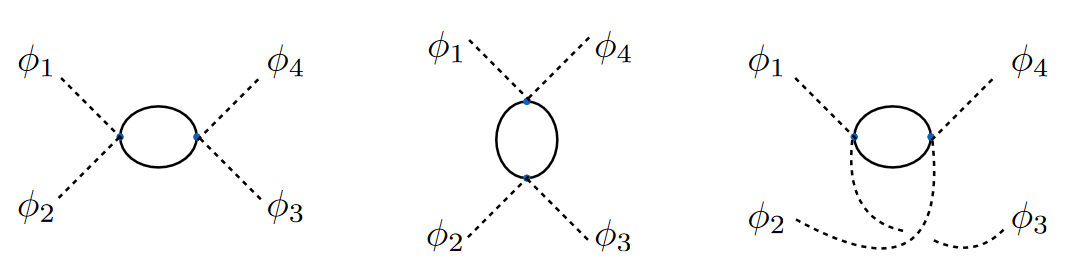
\includegraphics{2019/02/20190212_skinnerquartic.png}
\end{center}
which correspond to an amplitude
\begin{equation}
    \frac{\lambda^2}{2} \int^\Lambda \frac{d^4k}{(2\pi)^4}\frac{1}{k^2+m^2} \bkt{
        \frac{1}{(p_1+p_2+k)^2 +m^2}
        +\frac{1}{(p_1+p_4+k)^2+m^2}
        +\frac{1}{(p_1+p_3+k)^2+m^2}
    }.
\end{equation}
The overall factor of $1/2$ is a symmetry factor since the two internal lines are identical and can be exchanged, and the propagators can be read off by conservation of momentum at each vertex (taking all external momenta to be flowing in). We see that this integral goes as $d^4k/k^4$, so we expect a $\log\Lambda$ divergence. More precisely, the large $k$ behavior (where we care about this divergence) will look like%
    \footnote{This integral isn't totally immediate. To evaluate this, rewrite $k^3 dk= \frac{1}{2}k^2 d(k^2)$. Next, divide through in the numerator and denominator by $m^4$ to get
    \begin{equation*}
        \frac{1}{2}\int_0^\Lambda \frac{(k^2/m^2) d(k^2/m^2)}{(k^2/m^2) +1)^2}=\frac{1}{2}\int_0^{\Lambda^2/m^2} \frac{u\,du}{(u+1)^2}.
    \end{equation*}
    Finally, to evaluate the $u$ integral, just integrate by parts. Some similar integrals like $\int \frac{u\, du}{1+u}$ are amenable to a simple rewriting as $\frac{u}{1+u}=1-\frac{1}{1+u}$, but in general you'll want to integrate by parts:
    \begin{equation*}
        \int_0^{\Lambda^2/m^2} u\frac{du}{(1+u)^2}= -\left.\frac{u}{1+u}\right\rvert_0^{\Lambda^2/m^2} -\int \paren{-\frac{1}{1+u}}du=-\left.\frac{u}{1+u}\right\rvert_0^{\Lambda^2/m^2} +\left.\log(1+u)\right\rvert_0^{\Lambda^2/m^2}=\log\paren{1+\frac{\Lambda^2}{m^2}}-\frac{\Lambda^2}{\Lambda^2+m^2}.
    \end{equation*}
    
    }
\begin{align}
    \frac{3\lambda^2}{2} \int^\Lambda \frac{d^4k}{(2\pi)^4}\frac{1}{(k^2+m^2)^2} &= \frac{3\lambda^2}{16\pi^3} \int_0^\Lambda \frac{k^3 dk}{(k^2+m^2)^2}\\
    &= \frac{3\lambda^2}{32\pi^2} \int_0^{\Lambda^2/m^2} \frac{u\,du}{(1+u)^2}\\
    &= \frac{3\lambda^2}{32\pi^2} \bkt{
        \log\paren{1+\frac{\Lambda^2}{m^2}}-\frac{\Lambda^2}{\Lambda^2+m^2}\label{quarticdivergence}
    }.
\end{align}
This value is the shift in the $\lambda$ coupling before we introduce the $\delta \lambda$ counterterm.
If we then choose
\begin{equation}
    \delta \lambda =\frac{3\lambda^2}{32\pi^2} \bkt{\log \frac{\Lambda^2}{m^2}-1},
\end{equation}
we can then produce an effective coupling of 
\begin{equation}
    \lambda_{\text{eff}}=\lambda -\frac{3\lambda^2}{32\pi^2} \bkt{\log \paren{1+\frac{m^2}{\Lambda^2}}+\frac{m^2}{m^2+\Lambda^2}},
\end{equation}
which is finite as $\Lambda\to\infty$.%
    \footnote{
        This is just $\lambda$ plus the one-loop correction we computed to be \ref{quarticdivergence} plus our choice of $\delta \lambda$ (which is itself treated as a one-loop correction). In fact, we've neglected an overall minus sign in computing the one-loop correction. We should add a factor of $-i$ for the loop, and get rid of the $i$ as part of the overall momentum-conserving delta function which we've already dropped. Thus
        \begin{align*}
            \lambda_\text{eff}&=\lambda -\frac{3\lambda^2}{32\pi^2} \bkt{
                \log\paren{1+\frac{\Lambda^2}{m^2}}-\frac{\Lambda^2}{\Lambda^2+m^2}
            }
            +\frac{3\lambda^2}{32\pi^2} \bkt{\log \frac{\Lambda^2}{m^2}-1}\\
            &= \lambda -\frac{3\lambda^2}{32\pi^2} \bkt{\log \paren{1+\frac{m^2}{\Lambda^2}}+\frac{m^2}{m^2+\Lambda^2}}.
        \end{align*}
    }

For this next discussion, we'll need a trick due to Feynman:
\begin{equation}
    \int_0^1 \frac{dx}{\bkt{xA+(1-x)B}^2} =\frac{1}{B-1} \bkt{\frac{1}{xA+(1-x)B}}_0^1 = \frac{1}{AB}.
\end{equation}
We'll use this to rewrite products of denominators as these sorts of integrals, i.e. from right to left. Note that the integral can be put in a more manifestly symmetric form as
\begin{equation*}
    \int_0^1 dx \int_0^1 dy \frac{\delta(x+y-1)}{(xA+yB)^2}.
\end{equation*}

For our first diagram, let $p_{12}\equiv p_1 +p_2$. Then the propagators take the form
\begin{align*}
    \frac{1}{(p_{12}+k)^2+m^2}\frac{1}{k^2+m^2}&=\int_0^1 \frac{dx}{\bkt{x((p_{12}+k)^2+m^2)+(1-x)(k^2+m^2)}^2
    }\\
        &= \int_0^1 \frac{dx}{\bkt{(k+xp_{12})^2 +m^2 +x(1-x)p_{12}^2}^2}\\
        &= \int_0^1 \frac{dx}{\bkt{l^2+m^2+x(1-x)p_{12}^2}^2}
\end{align*}
where we have defined $l=k+x p_{12}.$
In the $\Lambda \to \infty$ limit, the shifted integration range $|k|\leq \Lambda \to |l|\leq \Lambda$ vanishes, so we can turn our $d^4k$ integral into a $d^4 l$ and write
\begin{align*}
    \int \frac{d^4ldx}
    {\bkt{l^2+m^2+x(1-x)p_{12}^2}^2}
    &= S_4 \int_0^1 dx \int_0^\Lambda \frac{l^3 dl}
    {\bkt{l^2+m^2+x(1-x)p_{12}^2}^2}\\
    &= \pi \int_0^1 dx \set*{ \log \bkt{
        \frac{\Lambda^2 +m^2+x(1-x)p_{12}^2}{m^2+m^2+x(1-x)p_{12}^2}
    }
    +\frac{m^2+x(1-x)p_{12}^2}{\Lambda^2+m^2+x(1-x)p_{12}^2}
    -1
    }
\end{align*}
after a change of variables and an integration by parts. Note that this term with the $1/\Lambda^2$ goes to zero as $\Lambda\to\infty$. Let's notice that all three diagrams are related by the Mandelstam variables 
\begin{equation}
    s=-(p_1+p_2)^2,t=-(p_1+p_4)^2,u=-(p_1+p_3)^2,
\end{equation}
so that the sum of our three diagrams is then
\begin{equation}
    \frac{\lambda^2}{32\pi^2}\int_0^1 dx \set*{ \log \paren{\frac{\Lambda^2}{m^2-x(1-x)s}} 
    + \log \paren{\frac{\Lambda^2} {m^2-x(1-x)t}}
    + \log \paren{\frac{\Lambda^2} {m^2-x(1-x)u}}
    -3
    }.
\end{equation}
The coefficient of $\tilde \phi^4$ in the effective action $\Gamma(\tilde \phi)$ (i.e. $\tilde \phi$ in momentum space) is
\begin{equation}
    \lambda+\delta \lambda -\frac{\lambda^2}{32\pi^2} \int d \set{\ldots}
\end{equation}
with $\delta \lambda$ from above, and replacing $(m^2,\lambda)\mapsto (m_{\text{phys}}^2,\lambda_{\text{eff}})$.
We find that 
\begin{equation}
    \lambda_{\text{eff}}+\frac{\lambda_{\text{eff}}^2}{32\pi^2} \int_0^1 dx \set*{ \log \bkt{1-\frac{x(1-x)s}{m_{\text{phys}}^2}}
    +\log \bkt{1-\frac{x(1-x)t}{m_{\text{phys}}^2}}
    +\log \bkt{1-\frac{x(1-x)u}{m_{\text{phys}}^2}}
    }
\end{equation}
is finite-- no more counterterms are necessary after $\delta m^2$ and $\delta \lambda$. Our capacity to regulate these terms depends on the idea of operators being relevant, irrelevant, or marginal (depending on their mass dimension as compared to the dimension of spacetime).

\section{Thursday, February 14, 2019}
    We've been looking at supersymmetric nonlinear sigma models. Previously, our fields were maps from $x:M\to N$ where $M$ was a worldline and $N$ was some target space, a Riemannian manifold with a metric $g$. But it's clear that $M$ could be some bigger manifold, in general ``our universe.''

We said the Hilbert space for our theory was
\begin{equation}
    \cH = \cH_x \otimes \cH_\psi = \Omega^\cdot (N,\CC),
\end{equation}
the space of differential forms up to $p$-forms on $N$ equipped with inner product
\begin{equation}
    \braket{\alpha}{\beta} = \int_N \bar \alpha \wedge * \beta,
\end{equation}
where $*$ is the Hodge star operator taking $\Omega^p(N)\to \Omega^{n-p}(N)$. Explicitly, if 
\begin{equation*}
    \omega=\omega_{a_1a_2\ldots a_p}dx^{a_1}\wedge dx^{a_2}\wedge \ldots \wedge dx^{a_p},
\end{equation*} then $*\omega$ is given by
\begin{equation*}
    *\omega =\frac{\sqrt{g}}{(n-p)!} \epsilon^{a_1\ldots a_p}{}_{b_{p+1} \ldots b_n} \omega_{a_1\ldots a_p} dx^{b_{p+1}}\wedge \ldots \wedge dx^{b_n},
\end{equation*}
with indices raised by the inverse metric. We saw that our SUSY operator $Q$ then has the geometric interpretation of an exterior derivative,
\begin{equation}
    \hat Q = i\hat{\bar \psi}^a \hat p_a \leftrightarrow d,
\end{equation}
and similarly $\hat{\bar Q}$ has the interpretation of the adjoint of the exterior derivative,
\begin{equation}
    \hat {\bar Q} = -i\hat{ \psi}^a \hat p_a \leftrightarrow d^\dagger,
\end{equation}
where $\avg{\alpha,d^\dagger \beta}=\avg{d\alpha,\beta}$.

We can now fix the ordering ambiguity in $|hat H$ by demanding the SUSY algebra
\begin{equation}
2\hat H=\set{\hat Q,\hat{\bar Q}}
\end{equation}
still holds in the quantum theory. This fixes
\begin{equation}
    H=\frac{1}{2} (d^\dagger d+ dd^\dagger)=-\frac{1}{2} \Delta,
\end{equation}
where $\Delta$ is the Laplacian acting on forms. Since $d:\Omega^p \to \Omega^{p+1}, d^\dagger: \Omega^p \to \Omega^{p-1},$ it follows that $-\Delta=d^\dagger d+dd^\dagger: \Omega^p \to \Omega^p$.

To see this concretely, when acting on a function $f\in \Omega^0(N)$ (i.e. a zero-form), $d^\dagger$ simply annihilates the function (since there are no $-1$-forms) so we get
\begin{align*}
    -\Delta f &= d^\dagger d f\\
        &= d^\dagger(\p_a f dx^a)\\
        &= *d(*df)\\
        &=*d \paren{
            \frac{\sqrt{g}}{(n-1)!} g^{ab} \p_a f \epsilon_{bc\ldots d} \underbrace{dx^c \wedge \ldots \wedge dx^d}_{n-1}
        }\\
        &=\frac{*}{(n-1)!} \p_m (\sqrt{g}g^{ab} \p_a f) \epsilon_{bc\ldots d} \underbrace{dx^m \wedge dx^c \wedge \ldots \wedge dx^d}_n.
\end{align*}
But we see that there are now $n$ one-forms being wedged together, which means we must have all the $dx^1$ through $dx^n$ in some order. We can rewrite this as a totally antisymmetric tensor, with a factor of $1/g$ the determinant of the metric. Using this fact, our expression becomes
\begin{align*}
    -\Delta f&=\frac{1}{g} \p_b(g^{ab}\sqrt{g} \p_a f)*(dx^1 \wedge \ldots \wedge dx^n)\\
    &= -\frac{1}{\sqrt{g}} \p_a(\sqrt{g} g^{ab} \p_b f).
\end{align*}
What we learn is that the generalized Laplacian acting on forms reduces to the ordinary Laplacian with respect to the metric when acting on functions.

However, we now observe that acting on any form $\omega$, 
\begin{align*}
    2\bra{\omega} \hat H \ket{\omega} &= \braket{\omega}{dd^\dagger \omega} + \braket{\omega}{d^\dagger d\omega}\\
        &= ||d^\dagger \omega||^2 + ||d\omega||^2 \geq 0.
\end{align*}
A form which has equality here, $\Delta \omega = 0$, is said to be \term{harmonic}. Therefore supersymmetric ground states are in $1:1$ correspondence with $\text{Harm}^\cdot (N) = \oplus_{p=0}^n \text{Harm}^p(N)$, the space of harmonic $0$- through $p$-forms on $N$. Notice that any form $\omega \in \text{Harm}^p$ must be closed ($d\omega=0$) and co-closed ($d^\dagger \omega=0$).

\begin{thm}[Hodge's theorem] The space of harmonic $p$-forms on $N$ is in correspondence with the de Rham $p$-cohomology group,
\begin{equation}
    \text{\emph{Harm}}^p(N) \cong H^p_{dR}(N)
\end{equation}
where
\begin{equation}
    H^p_{dR}(N)=\set{\omega \in \Omega^p(N)\text{ s.t. }d\omega=0}/\set{\omega=d\alpha} = \text{\emph{ker}}(d:\Omega^p\to \Omega^{p+1})/\text{\emph{im}}(d:\Omega^{p-1}\to \Omega^p).
\end{equation}
\end{thm}
In de Rham cohomology, $\omega$ is specified up to $\omega \sim \omega +d\alpha$ (i.e. we only care about $\omega$ up to the addition of some exact $d\alpha$). The role of the co-closure condition, $d^\dagger \omega=0$, is to select a unique representative. If $d\omega = d^\dagger \omega=0$, then we our freedom becomes $\omega \sim \omega +d\alpha$ where $d^\dagger d\alpha =0$, and the only solutions are $\alpha=0$.%
    \footnote{This is equivalent to the procedure in electromagnetism where we have a potential with a gauge symmetry $A\sim A+d\lambda$, and we fix the gauge by requiring that $d^\dagger A = \p^\mu A_\mu =0$.}
Thus the space of SUSY ground states is $\cong H^\cdot_{dR}(N)$.

Thinking back to our discussion of the Witten index, we see that
\begin{equation}
    I_W = \Tr((-1)^F e^{-\beta H}) = n_B -n_F =\sum_{p=0}^n (-1)^p \dim(H^p_{dR}(N)).
\end{equation}
But this is very interesting because this final expression is precisely $\chi(N)$, the \term{Euler character} of $N$. Thus the space of SUSY ground states has a close relation to some topological information about the space our states live in.

To motivate de Rham cohomology a bit more, suppose $C_p$ is a $p$-cycle in $N$ without boundary. Stokes's Theorem in the vector calculus language says that 
\begin{equation*}
    \int_S(\curl \vec A) \cdot d\vec S=\oint_C \vec A \cdot d\vec l.
\end{equation*}
But we can generalize this to $p$-forms:
\begin{equation}
    \int_{D_{p+1}} d\omega = \int_{C_p} \omega
\end{equation}
if $\p D_{p+1}=C_p$. That is, we can relate the integral in some region $D_{p+1}$ to the value of the form integrated over the boundary $C_p$. However, if $\omega\in H^p_{dR},$ then $d\omega=0 \implies \int \omega=0$ if $C_p$ is the boundary of some $D_{p+1}$.

Furthermore,
\begin{equation}
    \int_{C_p} \omega +d\alpha =\int_{D_{p+1}} d\omega + \int_{D_{p+1}} d^2 \alpha,
\end{equation}
where this second term vanishes since $d$ is nilpotent. Thus we arrive at de Rham's theorem:
\begin{thm}[de Rham]
    \begin{equation}
        H_{dR}^p(N) \cong H_p(N),
    \end{equation}
    where $H_p(N)$ denotes the $p$th homology group, the set \{$p$-cycles in $N$ with no boundary$\}/\{p$-cycles that are the boundary of some $(p+1)$-cycle\}.
\end{thm}

For instance, if $N=S^n$, then $\dim(H_{dR}^0(S^n))=1$. We can also find that  $\dim(H^p_{dR}(S^n))=0$ for $p\neq 0,n$ since we can contract any loop (e.g. an $S^1$) to a point on $S^n$. And then we have $\dim(H^n_{dR}(S^n))=1$, i.e. there is one non-trivial  ``wrapping'' of $S^n$ by an $S^n$.

For $n=\Sigma_g$ a handlebody with genus $n$ (i.e. $n$ donuts glued together) we have instead $H^0(\Sigma_g)=\CC$, $H^1(\Sigma_g)=\CC^{2g}$ and $H^2(\Sigma_g)=\CC$ (dimensions $1,2g,$ and $1$).

The Euler character for the $n$-sphere is
\begin{equation}
    \chi(S^n)=\begin{cases}
        2 & \text{if $n$ even}\\
        0 & \text{if $n$ odd},
    \end{cases}
\end{equation}
and for $\Sigma_g$ it is $\chi(\Sigma_g)=2-2g$.

For the path integral, $\chi(N)=\int e^{-S[x,\psi}\cD x \cD \psi \cD \bar \psi$, where all fields are periodic with period $\beta$. Now if we take the whole action, we see that our whole action is supersymmetrically trivial:
\begin{align}
    S &= \int \frac{1}{2} g_{ab} \dot x^a \dot x^b+\frac{1}{2} g_{ab} \bar \psi^a \nabla_t \psi^b + \frac{1}{4} R_{abcd} \bar \psi^a \psi^b \bar \psi^c \psi^d dt\\
    &= \bar Q \bkt{ \oint \frac{g_{ab} \bar \psi^a}{2}(i\dot x^b +\Gamma^b_{cd} \bar \psi^c \psi^d) dt.}
\end{align}
We therefore learn that the path integral is independent of $\beta$.

\section{Tuesday, February 19, 2019}
    Last time, we wrote down an action for the electromagnetic field,
\begin{equation*}
    S_g[A]=\frac{1}{4}\int d^4x F_{\mu\nu}F^{\mu\nu} = \frac{1}{2}\int\frac{d^4k}{(2\pi)^4} \tilde A_\mu(-k)(k^2\delta^{\mu\nu}-k^\mu k^\nu)\tilde A_\nu(k),
\end{equation*}
We introduced the Faddeev-Popov method for fixing the gauge. We write the identity in terms of a delta function and an (as yet unspecified) functional $G[A]$,
\begin{equation*}
    1= \int \cD \alpha(x) \delta (G[A]) \det \paren{\frac{\delta G[A]}{\delta \alpha}}.
\end{equation*}

For the $G[A]$ we will use, the determinant (Jacobian factor) will be independent of $A$, though this will not be true more generally in non-Abelian gauge theories. We can denote the gauge-transformed $A$ as
\begin{equation}
    A_\mu^\alpha(x)=A_\mu (x) +\frac{1}{e} \p_\mu \alpha(x).
\end{equation}
If we choose to work in Lorenz gauge, for example, then
\begin{equation}
    G[A]=\p_\mu A^\mu \implies G[A^\alpha]=\p_\mu A^\mu +\frac{1}{e} \p^2 \alpha,
\end{equation}
so
\begin{equation}
    \det \paren{\frac{\delta G[A]}{\delta \alpha}}=\det \paren{\frac{\p^2}{e}}.
\end{equation}
%what does this mean, notationally?
Thus we rewrite the path integral with our delta function as
\begin{align}
    \int \cD A e^{-S_g[A]} &= \det \paren{\frac{\delta G[A^\alpha]}{\delta \alpha}} \int \cD \alpha \int \cD A e^{-S_g[A]} \delta(G[A])\\
    &=\det \paren{\frac{\delta G[A^\alpha]}{\delta \alpha}} \paren{\int \cD \alpha} \int \cD A e^{-S_g[A]} \delta(G[A]),
\end{align}
where we have changed variables $A\mapsto A^\alpha$, and $S_g$ is invariant since this is a gauge transformation.%
    \footnote{n.b. this path integral over gauge transformations $\int \cD \alpha$ is infinite. It is the same infinity that cropped up when we tried to naively compute the full path integral before gauge fixing, but here we have isolated it with our gauge fixing procedure so it can be readily discarded.}

To fix the gauge, let's choose the functional
\begin{equation}
    G[A]=\p_\mu A^\mu(x) -\omega(x) \implies G[A^\alpha]=\p_\mu A^\mu - \omega +\frac{1}{e} \p^2 \alpha.
\end{equation}
We now integrate over $\omega$ with a Gaussian weight factor of mean $0$ and variance $\xi$. Thus
\begin{equation}
    \int \cD \omega \exp \bkt{-\int d^4x \frac{\omega^2}{2\xi}} \det \paren{\frac{\p^2}{e}} \int \cD \alpha \cD A e^{-S[A]}\delta(\p_\mu A^\mu -\omega),
\end{equation}
which becomes (similar to before)
\begin{equation}
    \det \paren{\frac{\p^2}{e}} \paren{\int \cD \alpha} \int \cD A e^{-S_g[A]}\exp \bigg(-\underbrace{\int d^4x \frac{1}{2\xi}(\p_\mu A^\mu)^2}_{S_{gf}[A]}\bigg),
\end{equation}
where $S_{gf}$ indicates a gauge-fixing action. Thus
\begin{equation}
    S_g[A]+S_{gf}[A]=\frac{1}{2} \int \frac{d^4k}{(2\pi)^k} \tilde A_\mu(-k) \bkt{k^2 \delta^{\mu\nu}-(1-\frac{1}{\xi})k^\mu k^\nu} \tilde A_\nu(k),
\end{equation}
where we've just taken a Fourier transform as usual. The propagator solves
\begin{equation}
    (k^2 \delta^{\mu\nu}-(1-\frac{1}{\xi})k^\mu k^\nu)\tilde D_{\nu\rho}(k)=\delta^\mu{}_\rho,
\end{equation}
so the photon propagator takes the form
\begin{equation}
    \tilde D^{\mu\nu}(k)=\frac{1}{k^2}\paren{ \delta^{\mu\nu}-(1-\xi) \frac{k^\nu k^\nu}{k^2}}.
\end{equation}
Here, $\xi=0$ is known as Lorenz or Landau gauge depending on when the $\xi$ condition is imposed, while $\xi=1$ is known as Feynman gauge.

\subsection*{Free fermions (electrons)}
Let us consider an action in terms of fermions,
\begin{equation}
    S[\psi,\bar \psi]=\int d^4x (-\bar \psi(\slashed{\p}+m)\psi),
\end{equation}
where we work in Euclidean signature, $\slashed{\p}=\gamma_\mu \p^\mu$, and the anticommutation relations hold,
\begin{equation}
    \set{\gamma_\mu,\gamma_\nu}=2\delta_{\mu\nu}.
\end{equation}
Our gamma matrices are hermitian, $\gamma_\mu^\dagger =\gamma_\mu$, and our $\gamma_5$ is taken to be $\gamma_5=\gamma_1 \gamma_2 \gamma_3 \gamma_4$. For example,
\begin{equation}
    \gamma_j=\begin{pmatrix}
        0& -i\sigma_j\\
        i\sigma_j & 0
    \end{pmatrix},
    \quad
    \gamma_4 = \begin{pmatrix}1 & 0 \\ 0 &-1\end{pmatrix}
    \text{ or } \begin{pmatrix}0 & 1 \\ 1 & 0\end{pmatrix}.
\end{equation}

We take the Fourier transform of our fermionic fields using
\begin{gather}
    \psi(x) =\int_p e^{ip\cdot x} \tilde \psi(p),\\
    \bar \psi(x) = \int_p e^{-ip\cdot x} \tilde{\bar \psi}(p)
\end{gather}
where $\int_p = \int \frac{d^4p}{(2\pi)^4}$. Thus in Fourier space our action takes the form
\begin{equation}
    S[\tilde \psi, \tilde{\bar \psi}]= \int_p \tilde{\bar \psi}(i\slashed{p}+m)\tilde \psi.
\end{equation}
Adding sources $\tilde \eta, \tilde{\bar \eta}$, the generating functional is then
\begin{align}
    Z[\tilde \eta,\tilde{\bar \eta}]&=\int \cD \tilde \psi \cD \tilde{\bar \psi} \exp \paren{-\int_p \bkt{ \tilde{\bar \psi}(i\slashed{p}+m)\tilde \psi - \tilde{\bar \eta} \tilde \psi +\tilde {\bar \psi}\tilde \eta}}\\
    &= Z[0,0] \exp\paren{-\int_p \tilde{\bar \eta}(i\slashed{p}+m)^{-1} \tilde \eta},
\end{align}
where we have completed the square as usual.

\subsection*{Feynman rules} In addition to the propagators and vertices, fermion loops pick up minus signs. For instance, the position space propagator takes the form
\begin{equation}
    S_F^{\alpha\beta}(x-y)=\avg{\psi^\alpha(x) \bar \psi^\beta(y)}=\int_p e^{ip \cdot(x-y)} \paren{\frac{1}{i \slashed{p}+m}}^{\alpha\beta},
\end{equation}
where $\alpha,\beta$ are spin indices $1,\ldots,4$. If we expand the action $e^{-S_{QED}}$ to second order in the electron-photon coupling, we find terms
\begin{align*}
    (-ie)^2 \avg{\paren{\int d^4x \bar \psi \slashed{A} \psi}\paren{\int d^4y \bar \psi \slashed{A} \psi}} &= (-ie)^2 \int d^4x d^4 y \,
    \avg{\slashed{A}^{\alpha\beta}(x) \slashed{A}^{\gamma\delta}(y) \bar \psi^\alpha(x) \psi^\beta(x) \bar \psi^\gamma(y) \psi^\delta(y)}.
\end{align*}
In general, we need to anticommute the $\psi$s and $\bar \psi$s to form propagators. One term is
\begin{equation}
    -(-ie)^2\int d^4x d^4y \,
    \paren{
        \slashed{A}^{\alpha\beta}(x) \slashed{A}^{\gamma\delta}(y) \underbrace{\psi^\beta(x) \bar \psi^\gamma(y)}_{S_F^{\beta\gamma}(x-y)} \underbrace{\psi^\delta(y) \bar \psi^\alpha(x)}_{S_F^{\delta \alpha}(y-x)}
    }
\end{equation}
where the overall minus sign comes from anticommuting and we've recognized the pairs $\psi \bar \psi$ as propagators.

We get some Feynman rules for this theory:
%see diagram
\begin{enumerate}
    \item The fermion propagator is an oriented line, with $\tilde S_F(p)=\frac{1}{i\slashed{p}+m}$
    \item The photon propagator is a squiggly line, $\tilde D^{\mu\nu}(k)=\frac{1}{k^2}(\delta^{\mu\nu}-(1-\xi)\frac{k^\mu k^\nu}{k^2})$
    \item The vertex gets a $-ie\gamma^\mu$.
    \item We pick up an overall factor of $(-1)^{l_F},$ where $l_F$ is the number of fermion loops.
\end{enumerate}
    
\section{Thursday, February 21, 2019}
    Last time, we considered fields in some spacetime and chose Gaussian normal coordinates in order to write (for variations of the fields $x^a=x^a_0+\delta x^a(\tau), \psi^a=\psi^a_0 +\delta \psi^a(\tau)$,
\begin{equation*}
    g_{ab}(x)=\delta_{ab} -\frac{1}{3} R_{acbd} (x_0) \delta x^c \delta x^d + O(\delta x^3)
\end{equation*}
and a connection
\begin{equation*}
    \Gamma^a_{bc}(x) = \p_d \Gamma^a_{bc}(x_0) \delta x^d = -\frac{1}{3} (R^a{}_{bcd}(x_0) +R^a{}_{cbd}(x_0))\delta x^d + O(\delta x^2).
\end{equation*}

So we have the quadratic action
\begin{equation}
    S^{(2)}[x_0,\psi_0,\delta x, \delta \psi]=\oint \paren{-\frac{1}{2} \delta x^a \delta_{ab} \frac{d^2}{d\tau^2}\delta x^b +\frac{1}{2} \delta \psi^a \delta_{ab} \frac{d}{d\tau} \delta \psi^b -\frac{1}{4} R_{abcd} \psi_0^a \psi_0^b \delta x^c \frac{d\delta x^d}{d\tau}} d\tau.
\end{equation}
For any fixed $(x_0^a,\psi_0^a)$, this is a free action, so the path integral over fluctuations gives
\begin{equation}
    \int e^{-S[x_0,\psi_0,\delta x , \delta \psi]}\cD \delta x \cD \delta \psi = \frac{\sqrt{\det'(\p_\tau \delta^b_a)}}{\sqrt{\det'(-\p^2\tau \delta^a_b - \mathcal{R}^a{}_b (x_0,\psi_0)\p_\tau)}}
\end{equation}
where $\mathcal{R}^a{}_b=R^a{}_{bcd}(x_0) \psi_0^c \psi_0^d$ and $\det'$ means without zero modes, i.e. we haven't yet done the integrals over $(x_0,\psi_0).$

We can split up the denominator by pulling out a $\p_\tau$ to find
\begin{equation}
    \int e^{-S[x_0,\psi_0,\delta x , \delta \psi]}\cD \delta x \cD \delta \psi = \frac{\sqrt{\det'(\p_\tau \delta^b_a)}}{\sqrt{\det'(\delta^a{}_b \p_\tau)}\sqrt{\det'(-\delta^a{}_b \p_\tau - \mathcal{R}_a{}^b)}}
    =\frac{1}{\sqrt{\det'(-\delta^a{}_b \p_\tau - \mathcal{R}^a{}_b)}}.
\end{equation}
Notice that the matrix $\mathcal{R}^a{}_b$ is an antisymmetric $n\times n$ matrix (since we contracted over two indices in the original Riemann tensor, and $R^a{}_{bcd}$ was already antisymmetric in the first two indices) and $n=2m$. We therefore decompose the tangent space $TN|_{x_0}$ into $m$ 2-dimensional subspaces on which $\mathcal{R}^a{}_b|_i$ takes the form
\begin{equation}
    \mathcal{R}^a{}_b|_i =\begin{pmatrix} 0 & \omega_i \\ -\omega_i & 0\end{pmatrix}.
\end{equation}
Let $-D_i$ be the restriction of $-\delta^a{}_b \p_\tau -\mathcal{R}^a{}_b$ to this 2D subspace.

We expand
\begin{equation}
    \delta x^a(\tau)=\sum_{k\neq 0} \delta x_k^a e^{2\pi i k \tau}.
\end{equation}
Then the eigenvalues of $-D_i$ on this subspace are $-2\pi i k \pm \omega_i$ for $k\in \ZZ,k\neq 0$ (where the first term comes from acting on a Fourier mode with $\p_\tau$ and the second comes the eigenvalues of $\mathcal{R}^a{}_b|_i$ being $\pm\omega$). Therefore
\begin{align*}
    \det(-D_i)&=\prod_{k\neq 0} (-2\pi i k+\omega_i)(-2\pi i k -\omega_i)\\
    &= \prod_{k\neq 0}(-(2\pi k)^2-\omega_i^2)\\
    &= \prod_{k=1}^\infty (2\pi k)^4 \prod_{k=1}^\infty \paren{1+\frac{\omega_i^2}{(2\pi k)^2}}^2,
\end{align*}
where the rewriting in the last line has come from changing the $k\neq 0$ product to a product over $k=1\to\infty$. 

This is clearly divergent thanks to the first factor. However, we can regularize this, e.g. using zeta-function regularization. We find that
\begin{equation}
    \prod_{k=1}^\infty (2\pi k)^4 = (4\pi^2)^{2\zeta(0)}e^{-2\zeta'(0)}=1.
\end{equation}
The important factor is then
\begin{equation*}
    \prod_{k=1}^\infty \paren{1+\frac{\omega_i^2}{(2\pi k)^2}}^2,
\end{equation*}
and we recall that 
\begin{equation*}
    \sinh(z)=z\prod_{k=1}^\infty \paren{1+\frac{z^2}{\pi^2 k^2}},
\end{equation*}
so after regularization, we have that $z=\omega_i^2/2$ and (by direct comparison with the expansion of $\sinh(z)$) our determinant term can be written as
\begin{equation}
    \sqrt{\det{}'(-D_i)}=\frac{\sinh(\omega_i/2)}{(\omega_i/2)}.
\end{equation}
We now see that
\begin{align}
    I_W&=\text{index}(\slashed\nabla)=\int \prod_{i=1}^\infty \frac{\omega_i/2}{\sinh(\omega_i/2)} d^n x_0 d^n\psi_0\\
        &= \int \det \paren{\frac{\mathcal{R}^a{}_b(x_0,\psi_0)/2}{\sinh(\mathcal{R}^a{}_b}(x_0,\psi_0)/2)}d^n x_0 d^n \psi_0.
\end{align}
where $\slashed{\nabla}$ denotes the Dirac operator on $N$. But by our regular Grassmann tricks, we must have precisely $n$ factors of $\psi_0$ in order for this integral to be non-vanishing. Thus
\begin{equation}
    I_W = \int_N \det \paren{\frac{\mathscr{R}/2}{\sinh \mathscr{R}/2}}.
\end{equation}
where $\mathscr{R}^a{}_b=R^a{}_{bcd}(x) dx^c \wedge dx^d$ is a curvature two-form. This is the Aatiyah-Singer index theorem.

\subsection*{Supersymmetric QFT}
If we had a $d$-dimensional theory that is Lorentz invariant, we must complete the supersymmetry algebra $\set{Q,Q^\dagger}=2H$. The Hamiltonian now comes with nontrivial kinetic terms and is part of the $d$-momentum multiplet $P_\mu$, so we need further supercharges. If we want to preserve $Q^\dagger =(Q)^\dagger$, then these supercharges must have the same spin, and so must each have spin $1/2$.

Specifically, the SUSY algebra in $d$-dimensions is
\begin{equation}
    \set{Q_\alpha,Q_\beta^\dagger}=2\gamma^\mu_{\alpha\beta} P_\mu,
\end{equation}
where $\alpha,\beta$ are spinor indices and $\gamma^\mu$ is a Dirac $\gamma$ matrix. We'll mostly be concerned with $d=2$, where Dirac spinors have $2^{(d/2)}=2$ complex components. Thus we can write $\psi=\begin{pmatrix}\psi_-\\\psi_+\end{pmatrix}$. With coordinates $(t,s)\in \RR^2$ and Minkowski metric $\eta_{\mu\nu}=\text{diag}(+,-)$, we can represent the Dirac $\gamma$s as
\begin{equation}
    \gamma^t = 
    \begin{pmatrix} 
    0 & 1\\
    1& 0
    \end{pmatrix},
    \quad
    \gamma^s = 
    \begin{pmatrix} 
    0 & -1\\
    1 & 0
    \end{pmatrix}.
\end{equation}
These obey the Clifford algebra $\set{\gamma^\mu, \gamma^\nu}=2\eta^{\mu\nu}$. The action for a free, massless Dirac spinor in $d=2$ is then
\begin{equation}
    S[\psi]=\frac{1}{2\pi}\int_{\RR^2} i\bar \psi \slashed{\p} \psi d^2 x
\end{equation}
where $\slashed{\p}=\gamma^\mu \p_\mu$ and $\bar \psi=\psi^\dagger \gamma^t$. We can of course plug in the explicit form of the spinors and $\gamma$ matrices, and we find that
\begin{equation}
    S[\psi]=\frac{1}{2\pi}\int {\RR^2} i\bar \psi_- (\p_t +\p_s)\psi_- +i\bar \psi_+(\p_t-\p_s)\psi_+ dtds,
\end{equation}
so we see that the spinor components decouple. Classically,
\begin{equation}
    (\p_t + \p_s)\psi_-=0\implies \psi_-(t,s)=f(t-s)
\end{equation}
represents a right-moving mode, while
\begin{equation}
    (\p_t - \p_s)\psi_+=0\implies \psi_+(t,s)=f(t+s)
\end{equation}
is a left-moving mode. Under an $SO(1,1)$ transformation, i.e.
\begin{equation}
    \begin{pmatrix}t\\ s\end{pmatrix} \mapsto
    \begin{pmatrix}
    \cosh\gamma & \sinh\gamma\\
    \sinh\gamma & \cosh\gamma
    \end{pmatrix}
    \begin{pmatrix}t\\ s\end{pmatrix}
\end{equation}
with $\gamma$ the usual (real) rapidity, the spinor components transform as
\begin{equation}
    \psi_\pm \mapsto e^{\pm \gamma/2}\psi,\quad \bar\psi_\pm \mapsto e^{\pm \gamma/2}\bar\psi.
\end{equation}

\section{Tuesday, February 26, 2019}
    \subsection*{Renormalization group}
Let's work with the action
\begin{equation}
    S_{\Lambda_0}[\phi]=\int d^dx\bkt{
        \frac{1}{2} \p_\mu \phi \p^\mu \phi +\sum_i \frac{1}{\Lambda_0^{d_i-d}} g_{i0} O_i(x)
    },
\end{equation}
where we're temporarily disregarding the mass coupling. The partition function $\cZ$ is then
\begin{equation}
    \cZ_{\Lambda_0}(g_{i0})=\int^{\Lambda_0} \cD \phi e^{-S_{\Lambda_0}[\phi]}.
\end{equation}
That is, we integrate over field configurations such that $|k|\leq \Lambda_0$. We might write the fields in terms of their Fourier transforms, i.e.
\begin{equation}
    \phi(x) = \int_{\abs{p}\leq \Lambda_0} \frac{d^dp}{(2\pi)^d} e^{ipx} \tilde \phi(p).
\end{equation}
Let us introduce $\Lambda < \Lambda_0$, a lower cutoff, and split the integral as
\begin{align*}
    \phi(x) &= \int_{\abs{p}\leq \Lambda} \frac{d^dp}{(2\pi)^d} e^{ipx} \tilde \phi(p) 
        +\int_{\Lambda < \abs{p}\leq \Lambda_0} \frac{d^dp}{(2\pi)^d} e^{ipx} \tilde \phi(p)\\
    &= \phi^-(x) + \phi^+(x).
\end{align*}
These sets of modes are disjoint, so we can write $\cD\phi = \cD \phi^- \cD \phi^+.$ Integrating over $\phi^+$ gives an effective action
\begin{equation}
    S_\Lambda^\text{eff}[\phi] = -\log \int_\Lambda^{\Lambda_0} \cD \phi^+ e^{-S_{\Lambda_0} [\phi^- + \phi^+]}.
\end{equation}
This ``RG equation'' tells us how to map $S_{\Lambda_0}\to S_\Lambda^{\text{eff}}$ as UV modes are integrated out, and this process can be iterated.%
    \footnote{
        In \emph{Statistical Field Theory}, we also had to rescale the momenta to match the original upper limit $\Lambda_0$ in order to study the ``same'' kind of theory. I'm not sure if we're just not interested in that here because we want an effective action, or if there's something else going on.
    }
We therefore write
\begin{equation}
    S_{\Lambda_0}[\phi^- + \phi^+] =S^0 [\phi^-]+S^0[\phi^+] + S_{\Lambda_0}^{\text{int}} [\phi^-,\phi^+]
\end{equation}
with free actions 
\begin{equation}
    S^0[\phi]=\int d^dx \,\frac{1}{2} \bkt{(\p \phi)^2 +m^2 \phi^2}.
\end{equation}
Note that since $\phi^-,\phi^+$ have disjoint support, there are no mixed $\phi^-\phi^+$ terms. Equivalently the Fourier transform of such a term would be $\tilde \phi^-(k) \tilde \phi^+(k')\delta(k+k')$, and since these modes are in different regions of momentum space, they will not mix. Note this will be different for higher-order couplings.

Performing our integration over UV modes, we get some effective interactions
\begin{equation}
    S_\Lambda^{\text{int}}[\phi^-] = -\log \int \cD \phi^+\,\exp \bkt{-S^0[\phi^+]-S_{\Lambda_0}^\text{int} [\phi^-,\phi^+]}.
\end{equation}

\subsection*{Running couplings}
Remember, our basic principle is that the physics at low energies must be independent of the cutoffs $\Lambda,\Lambda_0$. Therefore
\begin{equation}
    \int^\Lambda \cD \phi \,e^{-S_\Lambda^\text{eff}[\phi]}=
        \int^{\Lambda_0} \cD \phi \, e^{-S_{\Lambda_0}[\phi]}.
\end{equation}
It follows that after integration, we will have some new, modified couplings which depend on $\Lambda$. Thus
\begin{equation}
    \cZ_\Lambda(g_i(\Lambda))=\cZ_{\Lambda_0}(g_{i0};\Lambda_0).
\end{equation}
But since the RHS is independent of $\Lambda$, so is the LHS. This places some constraints on the ``flow'' of the coupling constants, which we call the \term{Callan-Symantzik equation}. It takes the form
\begin{equation}
    0=\Lambda \frac{d\cZ_\Lambda(g)}{d\Lambda} =\paren{\Lambda\P{}{\Lambda}|_{g_i}+\Lambda \P{g_i}{\Lambda}\P{}{g_i}|_\Lambda
    } \cZ_\Lambda(g).
\end{equation}
Now, $S_{\Lambda_0}$ is completely general, so $S_\Lambda^{\text{eff}}$ should have the same form. We write
\begin{equation}
    S_\Lambda^\text{eff}[\phi] = \int d^dx \bkt{
        \frac{Z_\Lambda}{2}(\p \phi)^2+\sum_i \frac{Z_n^{n_i/2}}{\Lambda^{d_i-d}} g_i(\Lambda)O_i(x)
    }.
\end{equation}
in terms of some new coefficients $g_i$.
Integrating may give a $Z_\Lambda \neq 1$ factor. LSZ therefore implies we want a canonically normalized kinetic term. Let $\phi^r=Z_\Lambda^{1/2}\phi$ be the renormalized field. The remaining variations describing the $\Lambda$ dependence are given by the $g_i(\Lambda)$.

We can associate some $\beta$-functions to this theory by
\begin{equation}
    \beta_i^\text{cl}=(d_i-d),\quad \beta_i^\text{q}=\Lambda \P{g_i}{\Lambda},
\end{equation}
where the superscripts indicate classical and quantum contributions. For example, $\phi^4$ theory in 4 dimensions with a cutoff $\Lambda_0$ has an action of the form
\begin{equation}
    S+S^{CT}=\int d^4x \bkt{\frac{1}{2}(1+\delta Z)(\p\phi)^2 +\frac{1}{2}(m^2+\delta m^2) \phi^2 +\frac{1}{4!}(\lambda+\delta \lambda) \phi^4
    }.
\end{equation}
At one loop, we used the on-shell scheme to fx $\delta Z =0$ and choose $\delta m^2$ such that $m^2=m^2_{\text{phys}}$. In the language of the renormalization group, we can write
\begin{equation}
    g_2(\Lambda_0)=\frac{1}{\Lambda_0^2}(m^2+\delta m^2)=g_{20} -\frac{\lambda}{32 \pi^2} \paren{1-g_{20} \log(1+\frac{1}{g_{20}}
    },
\end{equation}
which is $\Lambda$-independent. Similarly,
\begin{equation}
    g_4(\Lambda_0)=\lambda +\delta \lambda =g_{40} +\frac{3g_{40}^2}{32\pi} \paren{\log\frac{
    \Lambda_0^2}{m^2}-1
    }.
\end{equation}
With our rescaled field $\phi^r =Z_\Lambda^{1/2} \phi$ (here $Z_\Lambda=1$, but not generally) we set
\begin{align*}
    g_\text{eff} &= \left.\frac{\delta^{4}\Gamma[\tilde \phi^r]}{\delta \tilde \phi^r (p_1) \delta \phi^r (p_2) \delta \tilde \phi^r (p_3) \delta \tilde \phi^r(p_4)}\right|_{p_i=0},
\end{align*}
which we can write as our sum of one-loop diagrams as before, but with a factor of $Z_\Lambda^{-2}$ to account for that these variations are taken with respect to the renormalized field. We find that
\begin{equation}
    \frac{dg_\text{eff}}{d\Lambda}=0.
\end{equation}

\subsection*{Anomalous dimensions}
in general $\delta Z \neq 0$, which means that $Z_\Lambda =1 +\delta Z \neq 1$ and therefore the kinetic term will transform nontrivially under renormalization. The anomalous dimension of the field $\phi$ is given by
\begin{equation}
    \gamma_\phi \equiv -\frac{\Lambda}{2} \P{}{\Lambda} \log Z_\Lambda,
\end{equation}
which is a ``$\beta$-function'' for the kinetic term. In our last example this was identically zero.

For instance, look at the $n$-point correlation function
\begin{equation}
    \avg{\phi(x_1)\ldots \phi(x_n)}=Z_\Lambda^{-n/2} \avg{\phi^r(x_1)\ldots \phi^r(x_n)}.
\end{equation}
We focus on the 1PI $n$-point functions calculated by variations with respect to $\phi^r$:
\begin{equation}
    \Gamma_\Lambda^{(n)}(x_1,\ldots,x_n; g_i(\Lambda)) = \frac{\delta^n \Gamma}{\delta \phi^r(x_1)\ldots \delta \phi^r(x_n)}.
\end{equation}
The fact that our predictions must be independent of $\Lambda$ tell us that we get the same expectation values for $s\lambda$ as for $\Lambda$, with $0<s <1$. Thus
\begin{equation}
    Z_{s\Lambda}^{-n/2}\Gamma_{s\Lambda}^{(n)}(x_1,\ldots, x_n; g(s\Lambda)) = Z_\Lambda^{-n/2} \Gamma_\Lambda^{(n)}(x_1,\ldots,x_n; g(\Lambda)).
\end{equation}
Under an infinitesimal $\delta s=1-s$, we get
\begin{equation}
    0=\Lambda \frac{d}{d\Lambda} \Gamma_\Lambda^{(n)}(x_1,\ldots,x_n; g(\Lambda))=\paren{\Lambda\P{}{\Lambda}+\beta_i \P{}{g_i}+n\gamma_\phi}\Gamma_\Lambda^{(n)}(x_1,\ldots,x_n; g_i(\Lambda))
\end{equation}
where $\beta^i=\Lambda \P{g_i}{\Lambda}$ is the quantum $\beta$-function. This is called the \term{generalized Callan-Symanzik equation}.

\section{Thursday, February 28, 2019}
    \begin{note}
We report the following erratum. Last time, we wrote an action as $S+S^{CT}$, and tried to connect it to the Wilsonian flow. However, this action has a definite cutoff, whereas the renormalization group interpretation requires us to integrate from $\Lambda$ to $\Lambda_0$, so these aren't quite comparable.
\end{note}

Let us now return to our discussion of anomalous dimension.%
    \footnote{Cf. Tong \emph{Statistical Field Theory} \textsection 3.2.}
Last time, we wrote down the anomalous dimension of a field $\phi$, given by
\begin{equation}
    \gamma_\phi \equiv -\frac{\Lambda}{2} \P{}{\Lambda} \log Z_\Lambda,
\end{equation}
and we derived the generalized Callan-Symanzik equation,
\begin{equation}
    0=\Lambda \frac{d}{d\Lambda} \Gamma_\Lambda^{(n)}(x_1,\ldots,x_n; g(\Lambda))=\paren{\Lambda\P{}{\Lambda}+\beta_i \P{}{g_i}+n\gamma_\phi}\Gamma_\Lambda^{(n)}(x_1,\ldots,x_n; g_i(\Lambda)).
\end{equation}
Thus if we let $\Lambda'=s\Lambda$, the differentiating with respect to $s$ we have
\begin{equation}
    s \P{}{s} Z_{s\Lambda}^{-n/2}=-\frac{n}{2} Z_{s\Lambda}^{-n/2} s\P{}{s} \log Z_{s\Lambda}=n \gamma
\end{equation}
using $s\P{}{s} = \Lambda' \P{}{\Lambda'}$.

Our RG process is then as follows.
\begin{enumerate}
    \item Integrate out modes with momenta in $(s\Lambda,\Lambda)$.
    \item Rescale coordinates $x^\mu \mapsto x'{}^\mu = sx^\mu$ in order to keep the kinetic term canonically normalized, $\frac{1}{2} \int d^dx \frac{1}{2} \p_\mu \phi \p^\mu \phi$, so that
    \begin{equation}
        \phi^r(sx) = s^{1-d/2} \phi^r(x).
    \end{equation}
    The rest of the action is invariant if $\Lambda \to \Lambda/s$.
\end{enumerate}
Then
\begin{align*}
    \Gamma_\Lambda^{(n)}(x_1,\ldots, x_n ; g_i(\Lambda)) &=\paren{\frac{Z_\Lambda}{Z_{s\Lambda}}}^{n/2} \Gamma_{s\Lambda}^{(n)}(x_1,\ldots, x_n ; g_i(s\Lambda))\\
    &= \paren{s^{2-d} \frac{Z_\Lambda}{Z_{s\Lambda}} }^{n/2} \Gamma_\Lambda^{(n)} (sx_1,\ldots, sx_n; g_i (s\Lambda)).
\end{align*}
Note the values $g_i(s\Lambda)$ and $Z_{s\Lambda}$ do not change under rescaling. Now a relabeling $x_i \mapsto \frac{x_i}{s}$ yields
\begin{equation}
    \Gamma_\Lambda^{(n)}(x_1/s,\ldots, x_n/s; g_i(\Lambda))= \paren{s^{2-d} \frac{Z_\Lambda}{Z_{s\Lambda}} }^{n/2} \Gamma_\Lambda^{(n)} (x_1,\ldots, x_n; g_i (s\Lambda)).
\end{equation}
Thus we can think of a running coupling while integrating out high-momentum modes as equivalent to the same coupling under a scaling transformation. As $s\to 0$, we are integrating out more modes. On the LHS, we see the separation between points increasing $\frac{|x_i-x_j|}{s}\to \infty$ (flowing to the long-distance infrared behavior), whereas on the RHS the separation is fixed but the coupling is ``running'' to lower energy scales (becomes insensitive to UV phenomena).

For infinitesimal $\delta s= 1-s$ we can expand to linear order,
\begin{equation}
    \paren{s^{2-d} \frac{Z_\Lambda}{Z_{s\Lambda}}}^{1/2} = 1+\paren{\frac{d-2}{2}+\gamma_\phi}\delta s +\ldots
\end{equation}
and we see that the fields scale with mass dimension
\begin{equation}
    \frac{d-2}{2} +\gamma_\phi \equiv \Delta \phi,
\end{equation}
where there is an ``engineering dimension'' that we always get (and could have read off from the kinetic term), plus an ``anomalous dimension.'' These add up to make an overall scaling dimension $\Delta \phi$ which in general is not the engineering dimension.

\subsection*{RG flow}
The renormalization group process tells us how couplings run as we integrate out high momentum modes and flow to the IR. These trace out trajectories, lines in the space of coupling constants which are governed by $\beta$-functions. Remarkably, some theories flow to the same endpoints, and therefore share the same IR physics. This is known as universality.

Where do such theories end up? If they end somewhere, they must end at fixed points (critical points), i.e. points in the space of coupling constants $g_i=g_i^*$ such that
\begin{equation}
    \beta_i|_{g_i=g_i^*}=0 \forall i,
\end{equation}
where we now mean the full $\beta$-function, including classical and quantum contributions.

In $\phi^4$ theory, there's an easy fixed point to spot. This is the Gaussian fixed point, $g_j^*=0 \forall j$, which is a massless free theory with no mass. If there are no couplings, there's nothing to flow and the theory stays at the fixed point. There are also nontrivial fixed points which require $\beta^\text{cl}$ and $\beta^\text{q}$ to cancel, such as the Wilson-Fisher fixed point.

\subsection*{Scale invariance at fixed points} Let us note that at fixed points, the couplings $g_i^*$ must be independent of scale, and dimensionless functions of $g_i^*$ become constant, e.g. $\gamma_\phi(g_i^*)=\gamma_\phi^*$.

Consider Callan-Symanzik for $n=2$ at a fixed point. We have
\begin{equation}
    \Lambda \P{}{\Lambda} \Gamma_\Lambda^{(2)}(x,y) = -2 \gamma_\phi^* \Gamma^{(2)} (x,y).
\end{equation}
Lorentz invariance tells us that $\Gamma^{(2)}$ must be a function of $|x-y|$ only. Like $\avg{\phi(x)\phi(y)}$, $\Gamma^{(2)}$ has mass dimensions of $d-2$, so we posit that
\begin{equation}
    \Gamma_\Lambda^{(2)}(|x-y|; g_i^*) =\frac{\Lambda^{d-2}}{\Lambda^{2\Delta d}} \frac{c(g_i^*)}{|x-y|^{2\Delta d}}.
\end{equation}
%finish this

\section{Tuesday, March 5, 2019}
    \subsection*{Nonabelian gauge theories}
Today, we begin our discussion of nonabelian gauge theories. For an external reference, see Peskin and Schroeder or Osborn.

Notice that under a local $U(1)$ transformation of the fermion field 
\begin{equation}
    \psi(x)\mapsto e^{i\alpha(x)} \psi(x),
\end{equation}
the term $\bar \psi \slashed{\p}\psi$ is not invariant, since the derivative will generically hit the $x$ dependence in $e^{i\alpha (x)}$. Consider the derivative in the direction of $n^\mu$ a unit vector, i.e.
\begin{equation}
    n^\mu \p_\mu \psi = \lim_{a\to 0} \frac{1}{a} \bkt{\psi(x+an) - \psi(x)}.
\end{equation}
\begin{defn}
    A \term{parallel transporter} (aka \term{Wilson line}) is an object $U(y,x)$ with the following ($U(1)$) gauge transformation:
    \begin{equation}
        U(y,x)\mapsto e^{i\alpha(y)} U(y,x) e^{-i\alpha(x)}.
    \end{equation}
    If we also set $U(x,x)=1$, then $U(y,x)$ can be written as a phase
    \begin{equation}
        U(y,x)=e^{i\phi(y,x)},
    \end{equation}
    and we moreover take $U(x,y)=(U(y,x))^*$.
\end{defn}
With this Wilson line, we can define a covariant derivative for our theory,%
    \footnote{This should feel kind of like a Lie derivative. Rather than just naively comparing the field value at two points, as in the partial derivative, we're using parallel transport to drag the field to the same point, and then taking the infinitesimal limit.}
\begin{equation}
    n^\mu D_\mu \psi = \lim_{a\to 0} \frac{1}{a} \paren{\psi(x+an) -U(x+an,x) \psi(x)}
\end{equation}
such that
\begin{equation}
    \bar \psi n^\mu D_\mu \psi = \lim_{a\to 0} \frac{1}{a} \bkt{ \bar \psi_x \psi_{x+an}- \bar \psi_{x+an} \psi_x},
\end{equation}
which is gauge-invariant. For small $a$, define
\begin{align*}
    U(x+an,x) &= \exp \bkt{-iea n^\mu A_\mu(x+ \frac{a}{2}n) + O(a^3)}\\
        &= 1-ie an^\mu A_\mu(x+\frac{a}{2}n) +O(a^2),
\end{align*}
so our covariant derivative takes the familiar form
\begin{equation}
    D_\mu\psi(x)= \bkt{\p_\mu +ie A_\mu(x)} \psi(x),
\end{equation}
which is simply the minimal coupling of the gauge field $A_\mu(x)$.

Under gauge transformations,
\begin{gather}
    A_\mu(x) \mapsto A_\mu(x) -\frac{1}{e} \p_\mu \alpha(x)\\
    D_\mu \psi(x) \mapsto e^{i\alpha(x)}D_\mu \psi(x),
\end{gather}
which tells us that $D_\mu \psi$ transforms like $\psi$, as does $D_\nu (D_\mu \psi)$. We can consider how the commutator transforms under gauge transformations,
\begin{equation}
    [D_\mu,D_\nu]\psi \mapsto e^{i\alpha(x)} [D_\mu,D_\nu] \psi,
\end{equation}
where
\begin{equation}
    [D_\mu,D_\nu]=ie(\p_\mu A_\nu - \p_\nu A_\mu)\equiv ie F_{\mu\nu},
\end{equation}
the gauge-invariant field strength tensor.

Generally, our Lagrangian can contain terms which are Lorentz invariant like
\begin{equation}
    F_{\mu\nu} F^{\mu\nu}\text{ and } i\epsilon^{\mu\nu\rho\sigma} F_{\mu\nu} F_{\rho\sigma},
\end{equation}
though the latter term here breaks $P$ and $T$ symmetry. In terms of the parallel transporters $U$, the field strength tensor $F_{\mu\nu}$ emerges when we construct gauge-invariant \term{Wilson loops}, i.e. closed Wilson lines.%
    \footnote{As Osborn remarks, the parallel transporters are directly analogous to the equivalent construction in general relativity. The field strength tensor is really a sort of curvature, interpreted in this way. If you know the word holonomy, this is what that is.}
For instance, the plaquette, with overall value
\begin{equation}
    P_{12}(x)=U(y_1,y_4)U(y_4,y_3) U(y_3,y_2) U(y_2,y_1).
\end{equation}
We can expand this about small $a$ to find
\begin{equation}
    P_{12}(x)=1-iea^2 F_{12}(x)+ O(a^3)
\end{equation}

One can generalize this principle to a Lie group $G$ (e.g. $SU(N)$). The Lie group acts on our fields by local transformations,
\begin{equation}
    \psi(x) \mapsto V(x) \psi(x)
\end{equation}
with $V(x)$ in (a representation of) $G$, and Wilson lines then transform as
\begin{equation}
    U(y,x)\mapsto V(y) U(y,x) V^\dagger (x)
\end{equation}
with $U(x,x)=1$. In general there may be many gauge fields $A^a_\mu$, which transform under some representation of the Lie group. If $G$ has some (hermitian) generators $t^a$ in the Lie algebra $L(G)$ corresponding to $G$, then we can write the expansion of $U$ infinitesimally as
\begin{equation}
    U(x+an,x)=1+ig a n^\mu A_\mu^a t^a+O(a^2),
\end{equation}
where we take $g$ to be a coupling strength and
\begin{equation}
    [t^a,t^b] = if^{abc}t^c
\end{equation}
for $f^{abc}$ some structure constants which are totally antisymmetric in their indices. Note that the index $a$ is summed over (and should not be confused with the expansion parameter $a$). As we learned in \emph{Symmetries, Fields and Particles}, the Lie bracket obeys the Jacobi identity,
\begin{equation*}
    [t^a,[t^b,t^c]]+[t^b,[t^c,t^a]] +[t^c,[t^a,t^b]]=0.
\end{equation*}

To find the transformation of the $A^a$ gauge fields, we expand $V(x+an)$. Notice that $V(x) V^\dagger(x)=1$ (where we take $G$ to be unitary), so
\begin{align}
    V(x+an)V^\dagger(x) &= \bkt{(1+an^\mu \p_\mu +O(a^2))V(x)} V^\dagger (x)\\
        &= 1+an^\mu(\p_\mu V)V^\dagger+\ldots\\
        &=1-a n^\mu V(\p_\mu V^\dagger)+\ldots\label{vvdagger_infinitesimal},
\end{align}
where we have integrated by parts in the last line. 
Using this result and our expansion for $U(x+an,x)$, it follows that
\begin{align}
    V(x+an)U(x+an,x) V^\dagger(x) &= V(x+an)(1+ig an^\mu A_\mu^a t^a) V^\dagger(x)\nonumber\\
        &= V(x+an)V^\dagger(x) + V(x+an)(igan^\mu A_\mu^a t^a) V^\dagger(x)\nonumber\\
        &= 1- an^\mu V(x) \p_\mu V^\dagger(x) + V(x)(ig an^\mu A_\mu^a t^a) V^\dagger(x) +O(a^2)\nonumber\\
        &= 1+ iga n^\mu V(x) \paren{\frac{i}{g} \p_\mu +A_\mu^a t^a} V^\dagger(x).
\end{align}
Since
\begin{gather}
    U(x+an,x) \mapsto V(x+an)U(x+an,x) V^\dagger(x)\\
    \implies 1 + ig an^\mu A_\mu^a t^a \mapsto 1+ iga n^\mu V(x) \paren{\frac{i}{g} \p_\mu +A_\mu^a t^a} V^\dagger(x),
\end{gather}
we find by direct comparison that 
\begin{equation}
    A_\mu^a(x) t^a \mapsto V(x)\bkt{\frac{i}{g} \p_\mu+A_\mu^a(x) t^a} V^\dagger(x).
\end{equation}

Our covariant derivative is therefore
\begin{equation}
    D_\mu=\p_\mu -ig A_\mu^a t^a,
\end{equation}
and for infinitesimal transformations,
\begin{equation}
    V(x)=1+i\alpha^a t^a +O(\alpha^2)
\end{equation}
so that the field transformations are
\begin{gather}
    \psi(x) \mapsto (1+i\alpha^a(x) t^a) \psi(x)\\
    A_\mu^a(x) \mapsto A_\mu^a(x) +\frac{1}{g} \p_\mu \alpha^a(x) +f^{abc}A_\mu^b \alpha^c(x) = A_\mu^a+ \frac{1}{g} D_\mu \alpha^a.
\end{gather}
The field strength tensors $F^a_{\mu\nu}$ are then defined by the commutator
\begin{equation}
    [D_\mu,D_\nu]=-ig F_{\mu\nu}^a t^a
\end{equation}
with
\begin{equation}
    F_{\mu\nu}^a = \p_\mu A_\nu^a - \p_\nu A_\mu^a +g f^{abc}A_\mu^b A_\nu^c,
\end{equation}
where this last term reminds us that our Lie group is in general non-abelian. In electromagnetism, this last term vanished since the Lie group was abelian and thus the structure constants were all zero, and there was only a single $F_{\mu\nu}$ since $U(1)$ has one generator.

Under gauge transformations, the field strength tensor
\begin{equation}
    F_{\mu\nu}^a \mapsto F_{\mu\nu}^a - f^{abc}\alpha^b F_{\mu\nu}^c
\end{equation}
alone is not gauge invariant, but
\begin{equation}\label{fieldstrengthtrace}
    F_{\mu\nu}^a F^{a,\mu\nu} = \Tr F_{\mu\nu} F^{\mu\nu}
\end{equation}
is gauge invariant (where the trace is taken over generators indexed by $a$). Generically, the new term with the structure constants means that our theories will have self-interactions even at tree level.

\subsection*{Gauge fixing}
With our field strength tensor, we can write down a path integral
\begin{equation}
    \int \cD A \exp \bkt{-\frac{1}{4} \int d^4x \Tr F_{\mu\nu} F^{\mu\nu}},
\end{equation}
with the trace as in \ref{fieldstrengthtrace}. To quantize, we need to avoid integrating over configurations which are pure gauge (i.e. gauge-equivalent to $A_\mu(x)=0$). We do this through the Faddeev-Popov gauge fixing procedure, i.e. we set some $G[A]=0$ at each point $x$ such that
\begin{equation}
    1=\int \cD \alpha(x) \delta(G[A^\alpha]) \det \paren{\frac{\delta G[A^\alpha]}{\delta \alpha}}
\end{equation}
where $\alpha$ is not an index but instead parametrizes the gauge transformation, i.e.
\begin{equation}
    (A^\alpha)^a_\mu = A_\mu^a + \frac{1}{g} D_\mu \alpha^a.
\end{equation}
Note that for $G[A]$ linear in $A$, the variation $\frac{\delta G[A^\alpha]}{\delta \alpha}$ will be independent of $\alpha$. The gauge-fixing procedure is then as in QED:
\begin{enumerate}
    \item Intechange order of integration, $A\leftrightarrow \alpha$
    \item Change variables $A'=A^\alpha$, noting that $\cD A' =\cD A$
    \item Relabel (remove the $'$) and factor out the $\alpha$ integration (assuming linear $G[A]$).
\end{enumerate}
We arrive at
\begin{equation}
    \int \cD A e^{-S[A]}=\paren{\int \cD \alpha} \int \cD A e^{-S[A]} \delta(G[A]) \det \paren{\frac{\delta G[A^\alpha]}{\delta \alpha}}.
\end{equation}
Note that this final determinant can now depend on the gauge field $A$. We can calculate propagators similarly to QED, and we'll see that some new constraints emerge in our non-abelian theories.

\section{Thursday, March 7, 2019}
    \begin{quote}
    \textit{``Wald proved a version of the first law [of black hole mechanics] which is the most badass, hard version to prove.'' --Jorge Santos}
\end{quote}

In our last class, we talked about Killing horizons. We have seen that if $\cH^+$ is a Killing horizon with Killing vector field $\xi^a$, then
\begin{equation}
    \xi^a \nabla_a \xi^b|_{\cH^+} = \kappa_0 \xi^b.
\end{equation}
For the RN and Kerr-Newman solutions, the surface gravity $\kappa_0$ (which a priori could have been a function) is in fact a constant.

Hawking thought that perhaps we could prove that in general, the surface gravity was a constant and not dependent on where on the horizon we looked. This turns out to be true, and it leads us to the zeroth law of black hole mechanics.

\subsection*{Zeroth law}
\begin{prop}
    Consider a null geodesic congruence that contains the generators of a Killing horizon $\cN$. Then $\theta=\hat \sigma =\hat \omega=0$.
\end{prop}
\begin{proof}
    We know that $\hat \omega=0$ since our congruence is hypersurface orthogonal.%check Reall notes
    Let $\xi^a$ be a Killing field normal to $\cN$. On $\cN$, we can write $\xi^a= hU^a$, where $U^a$ is affinely parametrized and $h$ is a function on $\cN$.
    Let the horizon $\cN$ be specified by an equation $f=0$. Then we can write $U^a=h^{-1} \xi^a + f V^a$, where $V^a$ is a smooth vector field. This lets us extend $U^a$ off of $\cN$ a bit.
    
    We can calculate the optical matrix
    \begin{equation}
        B_{ab}=\nabla_b U_a = (\nabla_a h^{-1})\xi_a + h^{-1} \nabla_b \xi_a + (\nabla_b f)V_a +f \nabla_b V_a.
    \end{equation}
    Evaluating on $\cN$ and using the fact that $\xi$ is Killing,
    \begin{equation}
        B_{ab}|_\cN = \xi_{(a}\nabla_{b)} h^{-1} + V_{(a}\nabla_{b)}f|_{\cN},
    \end{equation}
    where we only consider the symmetric part since the antisymmetric part was $\omega$ and vanishes. But both $\xi_a,\nabla_a f$ are parallel to $U_a$ on $\cN$. Hence when we project onto $T_\perp$, we find that
    \begin{equation}
        \hat B_{(ab)}|_\cN = P_a{}^c B_{(cd)} P_b{}^d = 0,
    \end{equation}
    so indeed $\hat \sigma=0$.
\end{proof}

\begin{thm}[Zeroth law of black hole mechanics]
    $\kappa_0$ is constant on the future event horizon of a stationary black hole spacetime obeying the dominant energy condition.
\end{thm}
\begin{proof}
    Note that Hawking's theorem implies that $\cH^+$ is Killing with respect to some Killing vector field $\xi^a$. We have just seen that $\theta=0$ along the generators of $\cH^+$. Hence $\frac{d\theta}{d\lambda}=0$ (where $\lambda$ parametrizes the integral curves of the generators). We also have $\hat \sigma = \hat \omega =0$. Now the Raychaudhuri equation says that
    \begin{equation}
        0=R_{ab} \xi^a \xi^b|_{\cH^+} = 8\pi T_{ab} \xi^a \xi^b|_{\cH^+}
    \end{equation}
    where we've applied the Einstein equation and dropped the trace term since we're on the horizon.
    
    This implies that
    \begin{equation}
        J\cdot \xi|_{\cH^+} =0
    \end{equation}
    where $J_a \equiv -T_{ab}\xi^b$. Now $\xi^a$ is a future-directed causal vector, so by the dominant energy condition, $J_a$ is also future-directed. Hence the above equation implies that $J^a$ is parallel to $\xi^a$ on $\cH^+$.%revisit this?
    
    Since this is the case, we can look at the expression
    \begin{equation}
        0=\xi_{[a}J_{b]}|_{\cH^+}= -\frac{1}{8\pi} \xi_{[a} R_{b]c} \xi^c |_{\cH^+}.
    \end{equation}
    On Examples Sheet 4, problem 1, we will prove that the previous expression implies the following:
    \begin{equation}
        0=\frac{1}{8\pi} \xi_{[a}\nabla_{b]}\kappa_0|_{\cH^+}.
    \end{equation}
    But this means that $\nabla_a \kappa_0$ is proportional to $\xi_a$, i.e. 
    \begin{equation}
        t \cdot \nabla \kappa_0=0
    \end{equation}
    for any tangent vector to $\cH^+$. Hence $\kappa_0$ is constant on the horizon.
\end{proof}
In fact, one can relax the energy condition from the DEC a bit, but it requires other details about the spacetime (asymptotic flatness and others).

\subsection*{First law of black hole mechanics}
Consider the Kerr spacetime. The horizon area $A$ is the area of the intersection of $\cH^+$ with a partial Cauchy surface of $t={}$constant. It is also the area of the bifurcating Killing horizon. $A$ will be a function of $J$ and $M$, and we can consider the quantity $\frac{\kappa_0}{8\pi}$. This turns out to be
\begin{equation}
    \frac{\kappa_0}{8\pi}\delta A = \delta M -\Omega_H \delta J.
\end{equation}
This leads us to an interesting question. Start with a particular Kerr solution. Take a slice of the Kerr solution, perturb the initial conditions, and solve the perturbed initial value problem. Can we show that the area of the black hole increases in this way? This is hard to do and in fact wasn't completed until the 1990s.%Wald-- see Reall
%This is a version of the first law which is the most badass, hard version to prove.
However, there is a more physical argument we can make about this relationship, made much earlier by Hartle and others.

Suppose we have some matter with a stress-energy tensor of $O(\epsilon)$. That is, it is small compared to the stress-energy of the black hole. Let
\begin{equation}
    J^a = -T^a{}_b K^b,\quad L^a = T^a{}_b m^b
\end{equation}
where $K$ is the stationary Killing vector field and $m$ is the axisymmetric Killing vector field. We would like these currents to still be conserved after we throw some stuff in. In Kerr, $\nabla_a J^a$ is exactly zero. In the new metric, we have instead
\begin{equation}
    \nabla_a J^a = O(\epsilon^2), \nabla_a L^a = O(\epsilon^2)
\end{equation}
That is, the metric is perturbed from Kerr by $g=\bar g_K +\epsilon \hat g$ where $\bar g_K$ is exactly Kerr. Hence we get an $O(\epsilon)$ correction in the covariant derivative from the perturbation to the metric, and we get another factor of $\epsilon$ from the perturbation of the stress-energy tensor. Hence to order epsilon this really is a current.

One may compute (on examples sheet 3) that
\begin{equation}
    \delta M =-\int_\cN * J, \quad \delta J = -\int_\cN * L.
\end{equation}
Note that the $J$ in the first expression is the current corresponding to the Killing vector $K$, while the second $J$ is the angular momentum of the black hole.

Now, one may choose Gaussian null coordinates on the horizon. In these coordinates, $\cH^+$ is the surface $r=0$, and the metric on $\cH^+$ takes the form
\begin{equation}
     ds^2_{\cH^+}= 2drd\lambda +h_{ij}(\lambda,y) dy^i dy^j.
\end{equation}
Using $\sqrt{-g}=\sqrt{h}$, we can write
\begin{equation}
    \eta=\sqrt{h} d\lambda \wedge dr \wedge dy^1 \wedge dy^2
\end{equation}
and fix an orientation (i.e. choose whether or not to put a minus sign on our definition of $\eta$ as a volume element).

The orientation of $\cN$ used in defining $\delta M, \delta J$ is the one used in Stokes's theorem. Viewing $\cN$ as the boundary of the region with $r>0$ (the black hole exterior, if you like), the volume element on $\cN$ is $d\lambda \wedge dy^1 \wedge dy^2$. Hence on $\cN$,
\begin{equation}
    (*J)_{\lambda 12} = \sqrt{h} J^r = \sqrt{h} J_\lambda = \sqrt{h} U\cdot J
\end{equation}
where $U=\P{}{\lambda}$.

We can now evaluate everything on Kerr, since the deviation is $O(\epsilon^2)$. Hence $\cN$ is Killing with a killing vector $\xi=K+\Omega m$ on $\cN$, and we also have $\xi=f U$ for a function $f$. Using $\xi^a \nabla_a \xi^b|_{\cH^+}=\kappa_0 \xi^b$, we find that
\begin{equation}
    \xi \cdot \nabla( \log|f|)=\kappa_0 \implies f= \kappa_0 \lambda + f_0(y)
\end{equation}
(where we can integrate knowing $\kappa_0=0$).

So far, we have
\begin{equation}
     \xi^a = [\kappa_0 \lambda +f_0(y)]U^a,
\end{equation}
where $\lambda=0$ is the bifurcating surface. Hence we find that the integration constant vanishes, $f_0(y)=0$, and so
\begin{equation}
    \xi^a = \kappa_0 \lambda U^a\text{ on } \cN.
\end{equation}

From the definition of $\delta M$, we have (substituting)
\begin{align*}
    \delta M &= \int_\cN d\lambda d^2y \sqrt{h} T_{ab} U^a(\xi^b -\Omega_H m^b)\\
        &= \int_\cN d\lambda dy^2 \lambda \sqrt{h } T_{ab} U^a U^b \kappa_0 \lambda -\Omega_H \int_\cM d\lambda d^2y \sqrt{h} U\cdot L,
\end{align*}
where this second term is precisely $-\delta J$. However, we have not yet used the Einstein equation-- we can turn $T_{ab}$ into a curvature condition,
\begin{equation}
    8\pi T_{ab} U^a U^b = R_{ab} U^a U^b,
\end{equation}
so that
\begin{align*}
    \delta M -\Omega_H \delta J &= \frac{\kappa_0}{8\pi} \int_\cN d\lambda d^2 y \sqrt{h} \lambda R_{ab} U^a U^b\\
    \implies \delta M -\Omega_H \delta J &= -\frac{\kappa_0}{8\pi} \int d^2y \int_0^{+\infty} \sqrt{h} \lambda \frac{d\theta}{d\lambda} d\lambda\\
    &= -\frac{\kappa_0}{8\pi} \int d^2y \set*{ [\sqrt{h}\lambda\theta]_0^{+\infty} -\int_0^{+\infty}(\sqrt{h}+ \underbrace{\lambda \frac{d\sqrt{h}}{d\lambda}}_{O(\epsilon^2)})\theta d\lambda},
\end{align*}
where we applied Raychaudhuri and integrated by parts.

Now recall that
\begin{equation}
    \frac{d\sqrt{h}}{d\lambda}=\theta\sqrt{h}=O(\epsilon).
\end{equation}
We will assume the final states exist in a $\lambda\to +\infty$ limit, $\sqrt{h}$ is finite. Hence
\begin{equation}
    \int_0^{+\infty} \sqrt{h}\theta d\lambda = \int_0^{+\infty} \frac{d\sqrt{h}}{\lambda} d\lambda = \delta(\sqrt{h}).
\end{equation}
Finiteness gives $\theta = o(1/\lambda)$ (decays at least as fast as $1/\lambda$), and hence the boundary terms go away. We learn that
\begin{equation}
    \delta M-\Omega_H \delta J = \frac{\kappa_0}{8\pi} \delta A. \qed
\end{equation}
\end{document}